\part{Vectors and Tensors}
\section{Basics of Vectors}
\subsection{Vectors and Index Notation}
\begin{definition}{Vector, initial definition}{}
    A vector is an object with length and direction.
\end{definition}
One important types of vectors is displacement vectors, which point between points, \(A\) and \(B\), and are denoted \(\vv{a} = \vec{a} = \overrightarrow{AB}\).
Displacement vectors are free to move about under parallel displacements of both ends.
Another similar type is a position vectors which are fixed with one end at the origin, \(O\), and the other at some point, \(P\).
Position vectors are often denoted \(\vv{x} = \vec{x} = \overrightarrow{OP}\).

Normally we consider vectors in some specific basis.
In three dimensions a basis is formed of three linearly independent vectors.
The most common choice is of an orthonormal basis, \(\{\ve{i}\}\).
A basis is orthonormal if \(\abs{\ve{i}} = 1\) and \(\ve{i}\perp\ve{j}\) for all \(i\ne j\).
A basis is either right or left handed depending on the orientation of the vectors.
Typically we work with a right handed system.
Any vector can be expressed as a linear combination of basis vectors:
\[\vv{a} = a_1\ve{1} + a_2\ve{2} + a_3\ve{3} = (a_1, a_2, a_3).\]
The length of such a vector is then
\[\abs{\vv{a}} = a = \sqrt{a_1^2 + a_2^2 + a_3^2}.\]

To save writing lots of sums we use the Einstein summation convention.
Under this convention the following are equivalent:
\begin{align*}
    \vv{a} &= a_1\ve{1} + a_2\ve{2} + a_3\ve{3}\\
    &= \sum_{i=1}^{3} a_i\ve{i}\\
    &= a_i\ve{i}.
\end{align*}
The rules for the Einstein summation convention are as follows:
\begin{itemize}
    \item One index -- No sum, the indices present are said to be free indices and can take any value in \(\{1, 2, 3\}\).
    For example:
    \[a_i \in \{a_1, a_2, a_3\}, \qquad\text{or}\qquad a_i = b_i \iff a_1 = b_1 \wedge a_2 = b_2 \wedge a_3 = b_3.\]
    \item Two indices repeated -- Sum over the repeated index.
    For example:
    \[\vv{a} = a_i\ve{i} = a_1\ve{1} + a_2\ve{2} + a_3\ve{3}, \qquad\text{or}\qquad (A\vv{b})_i = A_{ij}b_j = A_{i1}b1 + A_{i2}b_2 + A_{i3}b_3.\]
    \item Three indices repeated -- Not allowed.
    For example
    \[(\vv{a}\cdot\vv{b})c_i = a_jb_jc_i \ne a_ib_ic_i, \qquad\text{or}\qquad (\vv{a}\cdot\vv{b})(\vv{c}\cdot\vv{d}) = a_ib_ic_jd_j \ne a_ib_ic_id_i\]
\end{itemize}

\subsection{Scalar Product}
The \define{scalar product}, or \define{dot product}, is a linear map taking two vectors to a scalar.
This map is symmetric and positive definite.
Formally a scalar product is defined as below:
\begin{definition}{Inner product}{}
    A real \define{inner product} or scalar product is a function, \(\cdot\colon V^2 \to \reals\), where \(V\) is a real vector space.
    The map must have the following properties:
    \begin{itemize}
        \item Linearity:
        \[(\alpha\vv{a})\cdot(\beta\vv{b}) = (\alpha\beta)(\vv{a}\cdot\vv{b})\qquad\text{and}\qquad (\vv{a} + \vv{b})\cdot\vv{c} = \vv{a}\cdot\vv{c} + \vv{b}\cdot\vv{c}.\]
        \item Symmetry:
        \[\vv{a}\cdot\vv{b} = \vv{b}\cdot\vv{a}.\]
        \item Positive-definiteness:
        \[\vv{a}\cdot\vv{a} \ge 0\]
        with equality only if \(\vv{a} = \vv{0}\).
    \end{itemize}
    One function that fits all of these properties, and is how we will define the scalar product, is
    \[\vv{a}\cdot\vv{b} = ab\cos\vartheta\]
    where \(\vartheta\) is the angle between \(\vv{a}\) and \(\vv{b}\).
\end{definition}
Notice that if \(\{\ve{i}\}\) is an orthonormal basis then
\[\ve{1}\cdot\ve{1} = \ve{2}\cdot\ve{2} = \ve{3}\cdot\ve{3} = 1\]
and 
\[\ve{1}\cdot\ve{2} = \ve{1}\cdot\ve{3} = \ve{2}\cdot\ve{3} = 0.\]
Using this and the properties of the scalar product we have that
\[\vv{a}\cdot\vv{b} = (a_i\ve{i})\cdot(b_j\ve{j}) = a_ib_j\ve{i}\cdot\ve{j}.\]
We define the \define{Kronecker delta} as
\[
\delta_{ij} = 
\begin{cases}
    1, & i = j,\\
    0, & i \ne j.
\end{cases}
\]
Which allows us to compactly write
\[\ve{i}\cdot\ve{j} = \delta_{ij}\]
and
\[\vv{a}\cdot\vv{b} = a_ib_j\delta_{ij}\]

If \(\vv{a}\) and \(\vv{b}\) are vectors and \(\vv{c} = \vv{b} - \vv{a}\) then
\[c^2 = \vv{c}\cdot\vv{c} = (\vv{b} - \vv{a})\cdot(\vv{b} - \vv{a}) = b^2 + a^2 - 2ab\cos\vartheta.\]
This is the \define{cosine rule}.
If we expand this in a different way then we get
\[\vv{c}\cdot\vv{c} = \vv{b}\cdot\vv{b} + \vv{a}\cdot\vv{a} - 2\vv{a}\cdot\vv{b}\]
\[\implies \vv{a}\cdot\vv{b} = \frac{1}{2}[\vv{b}\cdot\vv{b} + \vv{a}\cdot\vv{a} - \vv{c}\cdot\vv{c}]\]
\[\implies a_ib_j\delta_{ij} = \frac{1}{2}[b_1^2 + b_2^2 + b_3^2 + a_1^2 + a_2^2 + a_3^2 - (b_1 - a_1)^2 - (b_2 - a_2)^2 - (b_3 - a_3)^2] = a_1b_1 + a_2b_2 + a_3b_3 = a_ib_i.\]
Comparing the left and right hand side of this we see that
\[\delta_{ij}b_j = b_i.\] 

\subsection{Direction Cosines}
\begin{definition}{Direction cosines}{}
    Let \(\vartheta_i\) be the angle between \(\vv{a}\) and \(\ve{i}\).
    Then the \define{direction cosines} of \(\vv{a}\) are
    \[l_i = \cos\vartheta_i = \frac{a_i}{a}.\]
    The last equality is a result of \(a_i = \vv{a}\cdot\ve{i} = a\cos\vartheta\).
\end{definition}
Let \(\{l_i\}\) be the direction cosines of \(\vv{a}\) and \(\{m_i\}\) be the direction cosines of \(\vv{b}\).
Then
\[\cos\vartheta = \frac{\vv{a}\cdot\vv{b}}{ab} = \frac{a_i}{a}\frac{b_i}{b} = l_im_i.\]
By this we see that \(l_il_i = \vv{a}\cdot\vv{a} / a^2 = \cos(0) = 1\).

\subsection{Vector Product}
\begin{definition}{Vector product}{}
    The \define{vector product}, or \define{cross product}, of \(\vv{a}\) and \(\vv{b}\) is a linear map, \(\times\colon V^2\to V\) with the following properties:
    \begin{itemize}
        \item \(\vv{a} \times \vv{b} = \vv{0}\) if and only if \(\vv{a}\) and \(\vv{b}\) are collinear.
        \item \(\vv{a} \times \vv{b} = - \vv{b} \times \vv{a}\).
        \item The vector \(\vv{a}\times\vv{b}\) is perpendicular to both \(\vv{a}\) and \(\vv{b}\).
    \end{itemize}
    One function that fits this, which we shall use as the definition of the vector product, is
    \[\vv{a}\times\vv{b} = ab\sin(\vartheta)\vh{n}\]
    where \(\vh{n}\) is a unit vector perpendicular to \(\vv{a}\) and \(\vv{b}\) in such a way that \((\vv{a}, \vv{b}, \vh{n})\) is a right handed system.
\end{definition}
Notice that if \(\{\ve{i}\}\) is an orthonormal basis then
\[\ve{1}\times\ve{2} = \ve{3}, \qquad \ve{2}\times\ve{3} = \ve{1}, \qquad \ve{3}\times\ve{1} = \ve{2}\]
and
\[\ve{1}\times\ve{1} = \ve{2}\times\ve{2} = \ve{3}\times\ve{3} = \vv{0}.\]
If we define the \define{Levi--Civita} symbol as
\[
\varepsilon_{ijk} = 
\begin{cases}
    1, & (i, j, k)~\text{is an even permutation of}~(1, 2, 3),\\
    -1, & (i, j, k)~\text{is an odd permutation of}~(1, 2, 3),\\
    0, & \text{otherwise},
\end{cases}
\]
then we can compactly write
\[\ve{i}\times\ve{j} = \varepsilon_{ijk}\ve{k}.\]
For example
\begin{align*}
    \ve{1}\times\ve{2} &= \varepsilon_{12k}\ve{k}\\
    &= \varepsilon_{121}\ve{1} + \varepsilon_{122}\ve{2} + \varepsilon_{123}\ve{3}\\
    &= \ve{3},
\end{align*}
and
\begin{align*}
    \ve{2}\times\ve{1} &= \varepsilon_{21k}\ve{k}\\
    &= \varepsilon_{211}\ve{1} + \varepsilon_{212}\ve{2} + \varepsilon_{213}\ve{3}\\
    &= -\ve{3}.
\end{align*}
The cross product of two vectors, \(\vv{a}\) and \(\vv{b}\), is
\begin{align*}
    \vv{a}\times\vv{b} &= (a_1\ve{1} + a_2\ve{2} + a_3\ve{3})\times(b_1\ve{1} + b_2\ve{2} + b_3\ve{3})\\
    &= (a_2b_3 - a_3b_2)\ve{1} + (a_3b_1 - a_1b_3)\ve{2} + (a_1b_2 - a_2b_1)\ve{3}\\
    &= 
    \begin{pmatrix}
        a_2b_3 - a_3b_2\\
        a_3b_1 - a_1b_3\\
        a_1b_2 - a_2b_1
    \end{pmatrix}
    \\
    &=
    \begin{vmatrix}
        \ve{1} & \ve{2} & \ve{3}\\
        a_1 & a_2 & a_3\\
        b_1 & b_1 & b_3
    \end{vmatrix}
    \\
    &= (a_i\ve{i})\times(b_j\ve{j})\\
    &= \varepsilon_{ijk}a_ib_j\ve{k}
\end{align*}
Using the last part if we rename \((i, j, k)\rightarrow (j, k, i)\) we get \(\vv{a}\times\vv{b} = \varepsilon_{jki}a_jb_k\ve{i} = \varepsilon_{ijk}a_jb_k\ve{i}\) as \((j, k, i)\) is an even permutation of \((i, j, k)\).
Hence
\[(\vv{a}\times\vv{b})_i = \varepsilon_{ijk}a_jb_k.\]
For example:
\begin{align*}
    (\vv{a}\times\vv{b})_i &= \varepsilon_{ijk}a_jb_k\\
    &= \varepsilon_{111}a_1b_1 + \varepsilon_{112}a_1b_2 + \varepsilon_{113}a_1b_3\\
    &+ \varepsilon_{121}a_2b_1 + \varepsilon_{122}a_2b_2 + \varepsilon_{123}a_2b_3\\
    &+ \varepsilon_{131}a_3b_1 + \varepsilon_{132}a_3b_2 + \varepsilon_{133}a_3b_3\\
    &= \varepsilon_{123}a_2b_3 + \varepsilon_{132}a_3b_2\\
    &= a_2b_3  - a_3b_2.
\end{align*}

\section{Basics of Vector Calculus}
\subsection{More on the Vector Product}
The following are important properties of the vector product:
\begin{itemize}
    \item \(\vv{a} \times \vv{b} = \vv{0}\) if and only if \(\vv{a}\) and \(\vv{b}\) are co-linear.
    \item \(\vv{a} \times \vv{b} = -\vv{b} \times \vv{a}\), i.e. the vector product is anticommutative.
    \item \(\vv{a} \times \vv{b}\) is perpendicular to both \(\vv{a}\) and \(\vv{b}\).
    \item \((\vv{a} + \vv{b})\times \vv{c} = \vv{a}\times\vv{c} + \vv{b}\times\vv{c}\), i.e. the vector product distributes over addition.
    \item \((\alpha\vv{a})\times(\beta\vv{b}) = (\alpha\beta)(\vv{a}\times\vv{b})\) for all \(\alpha, \beta\in\reals\).
    This and the previous property make \(\times\) a linear operation.
    \item \(\vv{a}\times(\vv{b}\times\vv{c}) \ne (\vv{a}\times\vv{b})\times\vv{c}\), i.e. the vector product isn't associative.
    \item If \(\vv{w} = \vv{a} \times (\vv{b} \times \vv{c})\) then \(\vv{w}\) is in the plane defined by \(\vv{b}\) and \(\vv{c}\).
    \item If \(\vv{w'} = (\vv{a}\times\vv{b}) \times \vv{c}\) then \(\vv{w'}\) is in the plane defined by \(\vv{a}\) and \(\vv{b}\).
\end{itemize}
In the last two points by `is in the plane defined by \(\vv{a}\) and \(\vv{b}\)' we mean `is a linear combination of \(\vv{a}\) and \(\vv{b}\)'.
Exactly what the coefficients are is given by the next theorem:
\begin{theorem}{Vector triple product}{vector triple product}
    Let \(\vv{a}, \vv{b}, \vv{c} \in \reals^3\).
    Then
    \[\vv{a}\times(\vv{b}\times\vv{c}) = (\vv{a}\cdot\vv{c})\vv{b} - (\vv{a}\cdot\vv{b})\vv{c}\]
    and
    \[(\vv{a}\times\vv{b})\times\vv{c} = (\vv{a}\cdot\vv{c})\vv{b} - (\vv{b}\cdot\vv{c})\vv{a}.\]
\end{theorem}
\begin{proof}
    The vector \(\vv{b}\times\vv{c}\) is perpendicular to the plane defined by \(\vv{b}\) and \(\vv{c}\).
    This means that \(\vv{a}\times(\vv{b}\times\vv{c})\) is perpendicular to the perpendicular to the plane defined by \(\vv{b}\) and \(\vv{c}\).
    This means that \(\vv{a}\times(\vv{b}\times\vv{c})\) is in the plane defined by \(\vv{b}\) and \(\vv{c}\).
    Therefore there exists \(\beta, \gamma\in\reals\) such that
    \[\vv{a}\times(\vv{b}\times\vv{c}) = \beta\vv{b} + \gamma\vv{c}.\]
    Taking a scalar product with \(\vv{a}\) the left hand side of this becomes zero as \(\vv{a}\times(\vv{b}\times\vv{c})\) is perpendicular to \(\vv{a}\).
    The right hand side becomes
    \[0 = \beta(\vv{a}\cdot\vv{b}) + \gamma(\vv{a}\cdot\vv{c}) \implies \beta(\vv{a}\cdot\vv{b}) = -\gamma(\vv{a}\cdot\vv{c})\]
    Thus there exists \(\alpha\in\reals\) such that \(\beta = \alpha(\vv{a}\cdot\vv{c})\) and also \(\gamma = -\alpha(\vv{a}\cdot\vv{b})\).
    Therefore
    \[\vv{a}\times(\vv{b}\times\vv{c}) = \alpha[(\vv{a}\cdot\vv{c})\vv{b} - (\vv{a}\cdot\vv{b})\vv{c}].\]
    We can determine the value of \(\alpha\) by considering the specific case where \(\vv{a} = a\ve{y}\), \(\vv{b} = b\ve{x}\), and \(\vv{c} = c\ve{y}\).
    Then
    \[\vv{a}\times(\vv{b}\times\vv{c}) = abc\ve{y}\times(\ve{x}\times\ve{y}) = abc\ve{y}\times\ve{z} = abc\ve{x}\]
    and
    \[\alpha[(\vv{a}\cdot\vv{c})\vv{b} - (\vv{a}\cdot\vv{b})\vv{c}] = \alpha abc[(\ve{y}\cdot\ve{y})\ve{x} - (\ve{x}\cdot\ve{y})\ve{y}] = \alpha abc\ve{x}.\]
    Comparing these we see that \(\alpha = 1\) and hence
    \[\vv{a}\times(\vv{b}\times\vv{c}) = (\vv{a}\cdot\vv{c})\vv{b} - (\vv{a}\cdot\vv{b})\vv{c}.\]
    Finally
    \begin{align*}
        (\vv{a}\times\vv{b})\times\vv{c} &= -\vv{c}\times(\vv{a}\times\vv{b})\\
        &= (\vv{c}\cdot\vv{a})\vv{b} - (\vv{c}\cdot\vv{b})\vv{a}\\
        &= (\vv{a}\cdot\vv{c})\vv{b} - (\vv{b}\cdot\vv{c})\vv{a}.
    \end{align*}
\end{proof}
\begin{corollary}{Kronecker delta and Levi--Civita symbol relation}{}
    The following holds for all \(i, j, l, m \in \{1, 2, 3\}\):
    \[\varepsilon_{ijk}\varepsilon_{klm} = \delta_{il}\delta_{jm} - \delta_{im}\delta_{jl}.\]
\end{corollary}
\begin{proof}
    Let \(\vv{a}, \vv{b}, \vv{c}\in\reals^3\), then
    \begin{align*}
        [\vv{a}\times(\vv{b}\times\vv{c})]_i &= \varepsilon_{ijk}a_j(\vv{b}\times\vv{c})_k\\
        &= \varepsilon_{ijk}a_j(\varepsilon_{klm}b_lc_m)\\
        &= \varepsilon_{ijk}\varepsilon_{klm}a_jb_lc_m.
    \end{align*}
    Also by theorem~\ref{thm:vector triple product} we know that
    \begin{align*}
        [\vv{a}\times(\vv{b}\times\vv{c})]_i &= [(\vv{a}\cdot\vv{c})\vv{b} - (\vv{a}\cdot\vv{b})\vv{c}]_i\\
        &= a_jc_jb_i - a_jb_jc_i\\
        &= a_j\delta_{jm}c_mb_i - a_jb_j\delta_{im}c_m\\
        &= a_j\delta_{jm}c_m\delta_{il}b_l - a_j\delta_{jl}b_l\delta_{im}c_m\\
        &= (\delta_{il}\delta_{jm} = \delta_{im}\delta_{jl})a_jb_lc_m.
    \end{align*}
    Comparing these two expressions we see that
    \[\varepsilon_{ijk}\varepsilon_{klm} = \delta_{il}\delta_{jm} - \delta_{im}\delta_{jl}.\]
\end{proof}

\subsection{Fields}
\begin{definition}{Scalar and vector fields}{}
    A \define{field} is any function of position, \(f\colon\reals^3\to S\).
    We classify fields based on the type of their output.
    For example if \(S = \reals\) then we say \(f\) is a scalar field but if \(S = \reals^3\) then we say \(f\) is a vector field.
    That is a scalar (vector) field assigns a scalar (vector) to every point in space.
\end{definition}
Fields are incredibly common in physics.
For example the temperature at position \(\vv{r}\) is a field, \(T(\vv{r})\).
A common example of a vector field is the electric field, \(\vv{E}(\vv{r})\).

\subsection{Vector Calculus}
\begin{definition}{Gradient}{}
    Let \(\varphi\colon\reals^3\to\reals\) be a scalar field.
    Then the \define{gradient} of \(\varphi\) is the vector field, \(\grad\varphi\colon\reals^3\to\reals^3\), defined by
    \[\grad\varphi = \ve{x}\pdv{\varphi}{x} + \ve{y}\pdv{\varphi}{y} + \ve{z}\pdv{\varphi}{z} = \ve{i}\partial_i\varphi.\]
\end{definition}
We can view \(\grad\) as a vector with components \((\grad)_i = \partial_i\).
This makes it natural to consider scalar and vector products of \(\grad\) with other vectors.
\begin{definition}{Divergence}{}
    Let \(\vv{a}\colon\reals^3\to\reals^3\) be a vector field.
    Then the \define{divergence} of \(\vv{a}\) is the scalar field, \(\div\vv{a}\colon\reals^3\to\reals\), defined by
    \[\div\vv{a} = \pdv{a_x}{x} + \pdv{a_y}{y} + \pdv{a_z}{z} = \partial_ia_i.\]
\end{definition}
\begin{definition}{Curl}{}
    Let \(\vv{a}\colon\reals^3\to\reals^3\) be a vector field.
    Then the \define{curl} of \(\vv{a}\) is the vector field, \(\curl\vv{a}:\reals^3\to\reals^3\), defined by
    \begin{align*}
        \curl\vv{a} &= \left(\pdv{a_y}{z} - \pdv{a_z}{y}\right)\ve{x} + \left(\pdv{a_z}{x} - \pdv{a_x}{z}\right)\ve{y} + \left(\pdv{a_x}{y} - \pdv{a_y}{x}\right)\ve{z}\\
        &= 
        \begin{vmatrix}
            \ve{x} & \ve{y} & \ve{z}\\
            \partial_x & \partial_y & \partial_z\\
            a_x & a_y & a_z
        \end{vmatrix}
        \\
        &= \varepsilon_{ijk}\ve{i}\partial_ja_k
    \end{align*}
    or in terms of its components
    \[(\curl\vv{a})_i = \varepsilon_{ijk}\partial_ja_k.\]
\end{definition}
We can also combine \(\grad\) with itself, for example \(\div\grad = \laplacian\).
\begin{definition}{Laplacian}{}
    Let \(\varphi\colon\reals^3\to\reals\) be a scalar field.
    Then the \define{Laplacian} of \(\varphi\) is the scalar field, \(\laplacian\varphi\colon\reals^3\to\reals\), defined by
    \[\laplacian\varphi = \pdv[2]{\varphi}{x} + \pdv[2]{\varphi}{y} + \pdv[2]{\varphi}{z} = \partial_i\partial_i\varphi.\]
    If \(\vv{a}\colon\reals^3\to\reals^3\) is a vector field then the \define{Laplacian} of \(\vv{a}\) is the vector field, \(\laplacian\vv{a}\colon\reals^3\to\reals^3\) defined by
    \[\laplacian\vv{a} = \ve{i}\laplacian a_i\]
    Here \(\laplacian a_i\) is the Laplacian of a scalar field as defined above.
\end{definition}
\begin{example}
    \textit{What is \(\grad r\)?}
    
    We will work out the components:
    \begin{align*}
        (\grad r)_i &= \partial_i r\\
        &= \partial_i(x_1^2 + x_2^2 + x_3^2)^{1/2}\\
        &= 2x_i\frac{1}{2}(x_1^2 + x_2^2 + x_3^2)^{-1/2}\\
        &= \frac{x_i}{r}.
    \end{align*}
    Therefore
    \[\grad r = \ve{i}\partial_i r = \frac{x_i}{r}\ve{i} = \frac{\vv{r}}{r} = \vh{r}.\]
    
    \textit{Find \(\curl(\curl\vv{a})\).}
    
    Again we work out the components:
    \begin{align*}
        [\curl(\curl\vv{a})]_i &= \varepsilon_{ijk}\partial_j(\curl\vv{a})_k\\
        &= \varepsilon_{ijk}\varepsilon_{klm}\partial_j\partial_la_m\\
        &= (\delta_{il}\delta_{jm} - \delta_{im}\delta_{jl})\partial_j\partial_la_m\\
        &= \delta_{il}\delta_{jm}\partial_j\partial_la_m - \delta_{im}\delta_{jl}\partial_j\partial_la_m\\
        &= \partial_j\partial_ia_j - \partial_j\partial_ja_i\\
        &= \partial_i(\div\vv{a}) - (\div\grad)a_i\\
        &= [\grad(\div\vv{a}) - \laplacian\vv{a}]_i.
    \end{align*}
    Hence
    \[\curl(\curl\vv{a}) = \grad(\div\vv{a}) - \laplacian\vv{a}.\]
    This gives us a useful identity for the Laplacian of a vector field, \(\vv{a}\):
    \[\laplacian\vv{a} = \grad(\div\vv{a}) - \curl(\curl\vv{a}).\]
    
    \textit{What is \(\curl(\vv{a}\times\vv{b})\)?}
    
    Working out the components:
    \begin{align*}
        [\curl(\vv{a}\times\vv{b})]_i &= \varepsilon_{ijk}\partial_j(\vv{a}\times\vv{b})_k\\
        &= \varepsilon_{ijk}\varepsilon_{klm}\partial_ja_lb_m\\
        &= (\delta_{il}\delta_{jm} - \delta_{im}\delta_{jl})\partial_ja_lb_m\\
        &= (\delta_{il}\delta_{jm} - \delta_{im}\delta_{jl})a_l\partial_jb_m + (\delta_{il}\delta_{jm} - \delta_{im}\delta_{jl})b_m\partial_ja_l\\
        &= \delta_{il}\delta_{jm}a_l\partial_jb_m - \delta_{im}\delta_{jl}a_l\partial_jb_m + \delta_{il}\delta_{jm}b_m\partial_ja_l - \delta_{im}\delta_{jl}b_m\partial_ja_l\\
        &= a_i\partial_jb_j - a_j\partial_jb_i + b_j\partial_ja_i - b_i\partial_ja_j\\
        &= a_i(\div\vv{b}) - (\vv{a}\cdot\grad)b_i + (\vv{b}\cdot\grad)a_i - b_i(\div\vv{a})\\
        &= [\vv{a}(\div\vv{b}) - (\vv{a}\cdot\grad)\vv{b} + (\vv{b}\cdot\grad)\vv{a} - \vv{b}(\div\vv{a})]_i.
    \end{align*}
    Hence
    \[\curl(\vv{a}\times\vv{b}) = \vv{a}(\div\vv{b}) + (\vv{b}\cdot\grad)\vv{a} - \vv{b}(\div\vv{a}) - (\vv{a}\cdot\grad)\vv{b}.\]
\end{example}

\section{Matrices}
\begin{definition}{Matrix}{}
    A real \(n\times m\) \define{matrix}, \(A\), is a rectangular array of real numbers with \(n\) rows and \(m\) columns.
    \[
    A = 
    \begin{pmatrix}
        a_{11}     & a_{12}     & \dots  & a_{1, n-1}    & a_{1n} \\
        a_{21}     & a_{22}     & \dots  & a_{2, n-1}    & a_{2n} \\
        \vdots     & \vdots     & \ddots & \vdots & \vdots \\
        a_{m-1, 1} & a_{m-1, 2} & \dots  &  a_{m-1, n-1} & a_{m-1, n}\\
        a_{m1}     & a_m{2}     & \dots  &  a_{m, n-1}    & a_{mn}
    \end{pmatrix}
    = (a_{ij})
    \]
\end{definition}
\begin{notation*}{}
    In these notes I will use the notation \(\nxmMatrices{n}{m}{S}\) to denote the set of \(n\times m\) matrices with entries from the set \(S\).
    This set will almost always be the real numbers and most of the time we consider square \(3\times 3\) matrices so most matrices will be in \(\nxmMatrices{3}{3}{\reals}\).
\end{notation*}
\begin{notation*}{}
    Matrices will normally be written with capital letter, such as \(A\in\nxmMatrices{n}{m}{\reals}\).
    The elements will be written with the same letter but lowercase or the same letter uppercase with indices, such as \(a_{ij}\) or \(A_{ij}\).
    If we want to define \(A\) by its components, \(a_{ij}\), then we will write \(A = (a_{ij})\).
\end{notation*}
\begin{definition}{Addition and scalar multiplication of matrices}{}
    Let \(A, B \in \nxmMatrices{n}{m}{\reals}\).
    Then the \define{sum}, \(A + B\), is the \(n\times m\) matrix with elements
    \[(A + B)_{ij} = a_{ij} + b_{ij}.\]
    \define{Subtraction} is similarly defined as the \(n\times m\) matrix with elements
    \[(A - B)_{ij} = a_{ij} - b_{ij}.\]
    So we see that for addition and subtraction we simply add or subtract matching entries.
    Addition and subtraction aren't defined if \(A\) and \(B\) have different numbers of rows or columns.
    \define{Scalar multiplication} by \(\lambda\in\reals\) is defined as
    \[(\lambda A)_{ij} = \lambda a_{ij}.\]
    So for scalar multiplication we simply multiply all entries by the scalar.
\end{definition}
\begin{definition}{Square matrix}{}
    A \define{square matrix} is simply a a matrix in \(\nxmMatrices{n}{n}{\reals}\).
    Of particular interest is the set of \(3\times 3\) matrices, \(\nxmMatrices{3}{3}{\reals}\) as these are very common to describe transformations in the three-dimensional space we live in.
\end{definition}
\begin{definition}{Identity matrix}{}
    The \define{identity matrix} or \define{unit matrix} in \(n\)-dimensions is the matrix
    \[
    \ident = 
    \begin{pmatrix}
        1 & 0 & \dots & 0\\
        0 & 1 & \dots & 0\\
        \vdots & \vdots & \ddots & \vdots\\
        0 & 0 & \dots & 1
    \end{pmatrix}
    = (\delta_{ij}).
    \]
    In particular the three-dimensional identity matrix is
    \[
    \ident = 
    \begin{pmatrix}
        1 & 0 & 0\\
        0 & 1 & 0\\
        0 & 0 & 1
    \end{pmatrix}
    .
    \]
\end{definition}
\begin{notation*}{}
    The identity matrix is variously denoted as \(I\), \(\mathbb{I}\), \(\mathrm{id}\), \(1\), and \(\mathds{1}\).
    Sometimes a subscript, \(n\), or \(n\times n\), is attached to denote the dimension of the matrix, such as \(I_3\) or \(I_{3\times 3}\) for the \(3\time 3\) identity matrix.
\end{notation*}
\begin{notation*}{}
    A \define{diagonal matrix} is a square matrix where \(a_{ij} = 0\) if \(i \ne j\).
    These matrices are common enough that we define special notation, \(\diag\).
    If \(A\in\nxmMatrices{n}{m}{\reals}\) has \(a_{ii} = a_i\) then
    \[
    \diag(a_1, a_2, \dotsc, a_n) = \diag(\vv{a}) = 
    \begin{pmatrix}
        a_1 & 0 & \dots & 0\\
        0 & a_2 & \dots & 0\\
        \vdots & \vdots & \ddots & \vdots\\
        0 & 0 & \dots & a_n
    \end{pmatrix}
    .
    \]
    For example the three-dimensional identity matrix is
    \[\ident = \diag(1, 1, 1).\]
\end{notation*}
\begin{definition}{Trace}{}
    The \define{trace} of a square matrix, \(A \in\nxmMatrices{n}{n}{\reals}\), is defined as
    \[\Tr A = a_{ii} = \sum_{i=1}^{n} a_{ii}.\]
    For example \(\Tr \ident = \delta_{ii} = 3\).
\end{definition}
\begin{notation*}{}
    The trace of \(A\) is sometimes denoted \(\mathrm{trace}A\), \(\tr A\), or \(\Tr A\).
\end{notation*}
\begin{definition}{Transpose}{}
    The \define{transpose} of \(A\in\nxmMatrices{n}{m}{\reals}\) is \(A\trans\in\nxmMatrices{m}{n}{\reals}\) defined by
    \[(A\trans)_{ij} = A_{ji}.\]
    For example
    \[
    \begin{pmatrix}
        1 & 2 & 3\\
        4 & 5 & 6
    \end{pmatrix}
    \trans
    =
    \begin{pmatrix}
        1 & 4\\
        2 & 5\\
        3 & 6
    \end{pmatrix}
    \]
    If \(A\trans = A\) we say that \(A\) is \define{symmetric}.
    If \(A\trans = -A\) we say that \(A\) is \define{antisymmetric}.
    For example the following are symmetric and antisymmetric respectively:
    \[
    \begin{pmatrix}
        1 & 2 & 3\\
        2 & 4 & 5\\
        3 & 5 & 6
    \end{pmatrix}
    , \qquad\text{and}\qquad
    \begin{pmatrix}
        1 & 2 & 3\\
        -2 & 4 & 5\\
        -3 & -5 & 6
    \end{pmatrix}
    .
    \]
\end{definition}
\begin{notation}{}{}
    The transpose of \(A\) is sometimes denoted \(A^T\), \(A^{\mathrm{T}}\), \(A^{\mathrm{tr}}\), \(\tensor[^{\mathrm{T}}]{A}{}\), or \(A\trans\).
\end{notation}
Notice that \(\Tr(A\trans) = \Tr(A)\) since the main diagonal is not changed by transposition.
\subsection{Matrix Product}
\begin{definition}{Matrix product}{}
    For \(A\in\nxmMatrices{n}{m}{\reals}\) and \(B\in\nxmMatrices{m}{p}{\reals}\) the product \(C = AB\) is defined as the matrix \(C\in\nxmMatrices{n}{p}{\reals}\) with entries
    \[c_{ij} = a_{ik}b_{kj}.\]
    Note that the sum is over \(k = 1, \dotsc, m\).
    Products of matrices where the number of columns of the first matrix is not the same as the number of rows of the second matrix are not defined.
\end{definition}
\begin{theorem}{Matrix product associativity and distributivity}{}
    If \(A\), \(B\), and \(C\) are matrices such that the products \(A(BC)\) and \((AB)C\) are defined then the product is associative:
    \[A(BC) = (AB)C,\]
    meaning we can unambiguously write \(ABC\).
    If \(A\), \(B\), and \(C\) are matrices such that the sum \(B + C\) and the products \(AB\) and \(AC\) are defined then the matrix product is distributive over addition:
    \[A(B + C) = AB + AC.\]
\end{theorem}
\begin{proof}
    Assuming that the necessary products exist we have
    \begin{align*}
        [A(BC)]_{ij} &= a_{ik}[BC]_{kj}\\
        &= a_{ik}(b_{kl}c_{lj})\\
        &= (a_{ik}b_{kl})c_{lj}\\
        &= [AB]_{il}c_{lj}\\
        &= [(AB)C]_{ij}
    \end{align*}
    Assuming that multiplication of the elements is associative this shows \(A(BC) = (AB)C\).
    
    Again assuming that \(A\), \(B\), and \(C\) are such that all operations are defined we have
    \begin{align*}
        [A(B + C)]_{ij} &= a_{ik}[B + C]_{kj}\\
        &= a_{ik}(b_{kj} + c_{kj})\\
        &= a_{ik}b_{kj} + a_{ij}c_{kj}\\
        &= [AB + AC]_{ij}.
    \end{align*}
    Assuming that multiplication of the elements distributes over addition this shows that \(A(B + C) = AB + AC\).
\end{proof}
Matrix multiplication is not commutative.
For example if \(A\in\nxmMatrices{n}{m}{\reals}\) and \(B\in\nxmMatrices{m}{p}{\reals}\) and \(n \ne p\) then \(AB\) defined and \(BA\) isn't.
Even in the case that \(A, B \in \nxmMatrices{n}{n}{\reals}\) it isn't always the case that \(AB = BA\).
For example
\[
\begin{pmatrix}
    1 & 2\\
    3 & 4
\end{pmatrix}
\begin{pmatrix}
    5 & 6\\
    7 & 8
\end{pmatrix}
=
\begin{pmatrix}
    19 & 22\\
    43 & 50
\end{pmatrix}
\ne
\begin{pmatrix}
    23 & 34\\
    31 & 46
\end{pmatrix}
=
\begin{pmatrix}
    5 & 6\\
    7 & 8
\end{pmatrix}
\begin{pmatrix}
    1 & 2\\
    3 & 4
\end{pmatrix}
.
\]
\begin{lemma}{Transpose of a product}{}
    Let \(A\) and \(B\) be matrices such that \(AB\) is defined.
    Then \((AB)\trans = B\trans A\trans\).
\end{lemma}
\begin{proof}
    Let \(A\) and \(B\) be matrices such that \(AB\) is defined.
    Then
    \begin{align*}
        [(AB)\trans]_{ij} &= [AB]_{ji}\\
        &= a_{jk}b_{ki}\\
        &= b_{ki}a_{jk}\\
        &= [B]_{ki}[A]_{jk}\\
        &= [B\trans]_{ik}[A\trans]_{kj}\\
        &= [B\trans A\trans]_{ij}.
    \end{align*}
    Assuming that multiplication of elements is commutative this shows that \((AB)\trans = B\trans A\trans\).
\end{proof}

\subsection{Determinants}
\begin{definition}{Determinant}{}
    The \define{determinant} of a \(3\times 3\) matrix, \(A\), is defined as
    \[\det A = \abs{A} = \norm{A} = \varepsilon_{ijk}a_{1i}a_{2j}a_{3k}.\]
\end{definition}
The determinant can equivalently be defined by a recursive definition.
First we define the determinant of a \(2\times 2\) matrix, \(B\), to be
\[
\det B =
\begin{vmatrix}
    b_{11} & b_{12}\\
    b_{21} & b_{22}
\end{vmatrix}
= b_{11}b_{22} - b_{21}b_{12}
\]
and then
\begin{align*}
    \det A &= \begin{vmatrix}
        a_{11} & a_{12} & a_{13}\\
        a_{21} & a_{22} & a_{23}\\
        a_{31} & a_{32} & a_{33}
    \end{vmatrix}
    \\
    &= a_{11}
    \begin{vmatrix}
        a_{22} & a_{23}\\
        a_{32} & a_{33}
    \end{vmatrix}
    - a_{12}
    \begin{vmatrix}
        a_{21} & a_{23}\\
        a_{31} & a_{33}
    \end{vmatrix}
    + a_{13}
    \begin{vmatrix}
        a_{21} & a_{22}\\
        a_{31} & a_{32}
    \end{vmatrix}
    \\
    &= 
    a_{11}(a_{22}a_{33} - a_{23}a_{32}) - a_{12}(a_{21}a_{33} - a_{23}a_{31}) + a_{13}(a_{21}a_{32} - a_{22}a_{31}).
\end{align*}
The determinant generalises to \(n\times n\) matrices fairly easily.
If \(A\in\nxmMatrices{n}{n}{\reals}\) then
\[\det A = \varepsilon_{i_1i_2\dotsm i_n} a_{1i_1}a_{2i_2}\dotsm a_{ni_n}\]
where \(\varepsilon_{i_1i_2\dotsm i_n}\) is the \(n\)-dimensional Levi--Civita symbol defined by
\[
\varepsilon_{i_1i_2\dotsm i_n} =
\begin{cases}
    +1, & (i_1, i_2, \dotsc, i_n)~\text{is an even permutation of}~(1, 2, \dotsc, n),\\
    -1, & (i_1, i_2, \dotsc, i_n)~\text{is an odd permutation of}~(1, 2, \dotsc, n),\\
    0, & \text{otherwise}.
\end{cases}
\]
The recursive definition of the determinant can also be generalised to higher dimensions.
First we define the minor, \(M^{(i, j)}\), of the matrix \(A\in\nxmMatrices{n}{n}{\reals}\) to be the \((n-1)\times(n-1)\) matrix we get if we delete the \(i\)th row and \(j\)th column of \(A\).
Then
\[\det A = \sum_{i=1}^n (-1)^{i + j}a_{ij}\det M^{(i, j)} = \sum_{j=1}^{n} (-1)^{i+j} a_{ij}\det M^{(i, j)}.\]
Notice that we are free to choose any value of \(j\) in the first sum or any value of \(i\) in the second sum.
We can often use this to our benefit by expanding the sum in a row or column with a lot of zeros so that lots of terms vanish simplifying the calculation.
Usually it is easier to calculate a specific determinant with the recursive definition and to prove something involving determinants with the \(\varepsilon_{ijk}\) definition.

\section{Determinant Properties}
In the last section we saw that for \(A\in\nxmMatrices{3}{3}{\reals}\) the determinant is defined as
\[\det A = \varepsilon_{lmn}a_{1l}a_{2m}a_{3n}.\]
Now define
\[X_{ijk} = \varepsilon_{lmn}a_{il}a_{jm}a_{kn}.\]
Then we have
\begin{align*}
    X_{jik} &= \varepsilon_{lmn}a_{jl}a_{im}a_{kn} & \swap{l}{m}\\
    &= \varepsilon_{mln}a_{jm}a_{il}a_{kn} & \varepsilon_{mln} = -\varepsilon_{lmn}\\
    &= -\varepsilon_{lmn}a_{il}a_{jm}a_{kn}\\
    &= -X_{ijk}.
\end{align*}
Similarly we can show that \(X_{kji} = X_{ikj} = -X_{ijk}\) and \(X_{jki} = X_{kij} = X_{ijk}\).
We see that the symmetry of \(X_{ijk}\) is the same as the symmetry of \(\varepsilon_{ijk}\) so we can write \(X_{ijk} = c\varepsilon_{ijk}\) for some \(c\in\reals\).
To find \(c\) we consider the specific case \((i, j, k) = (1, 2, 3)\) and we see that
\[X_{123} = \varepsilon_{lmn}a_{1l}a_{2m}a_{3n} = \det A.\]
This means that \(X_{ijk} = \varepsilon_{ijk}\det A\), we conclude
\[\varepsilon_{ijk}\det A = \varepsilon_{lmn}a_{il}a_{jm}a_{kn}.\]
If we then use \(\varepsilon_{ijk}\varepsilon_{ijk} = 6\) we see that
\[\det A = \frac{1}{3!}\varepsilon_{ijk}\varepsilon_{lmn}a_{il}a_{jm}a_{kn}.\]
This is a symmetric form for the determinant.
This generalises to \(B\in\nxmMatrices{n}{n}{\reals}\) as
\[\det B = \frac{1}{n!}\varepsilon_{i_1i_2\dots i_n}\varepsilon_{j_1j_2\dotsm j_n}b_{i_1j_1}b_{i_2j_2}\dotsm b_{i_nj_n}.\]

If we define
\[Y_{lmn} = \varepsilon_{ijk}a_{il}a_{jm}a_{kn}\]
we see by the same argument that \(Y_{lmn} = \varepsilon_{lmn}Y_{123}\).
Further
\[\det A = \frac{1}{3!}\varepsilon_{ijk}\varepsilon_{lmn}a_{il}a_{jm}a_{kn} = \frac{1}{3!}\varepsilon_{lmn}Y_{lmn} = \frac{1}{3!}\varepsilon_{lmn}\varepsilon_{lmn}Y_{123} = Y_{123}.\]
So we have that
\[\det A = \varepsilon_{ijk}a_{i1}a_{j2}a_{k3}.\]
What this means is that we can expand along a column as well as a row when using the recursive definition of the determinant.
As well as this since \(Y_{lmn} = \varepsilon_{lmn}\det A\) we see that
\[\varepsilon_{lmn}\det A = \varepsilon_{ijk}a_{il}a_{jm}a_{kn}.\]

We will now list some properties of the determinant.
We won't prove these but will give examples.
\begin{itemize}
    \item If we multiply one row (or column) of \(A\) by a scalar, \(\lambda\in\reals\), to make the matrix \(A'\)  then \(\det A' = \lambda\det A\).
    For example suppose we multiply the first row by \(\lambda\) so \(a'_{1i} = \lambda a_{1i}\), \(a'_{ij} = a_{ij}\) for \(i = 2, 3\).
    Then
    \[\det A' = \varepsilon_{lmn}a'_{1l}a'_{2m}a'_{3n} = \varepsilon_{lmn}(\lambda a_{1l})a_{2m}a_{3n} = \lambda \det A.\]
    
    \item Multiplying an \(n\times n\) matrix by \(\lambda\in\reals\) multiplies the determinant by \(\lambda^n\).
    This follows by applying the previous point to each row individually multiplied by \(\lambda\).
    
    \item Adding a multiple of one row to another row (or a multiple of a column to another column) does not change the value of the determinant.
    For example if we add \(\lambda\) times the second row to the first row to get \(A'\) defined by \(a'_{1i} = a_{1i} + \lambda a_{2i}\) and \(a'_{ij} = a_{ij}\) for \(i = 2, 3\) then
    \[\det A' = \varepsilon_{lmn}a'_{1l}a'_{2m}a'_{3n} = \varepsilon_{lmn}(a_{1l} + \lambda a_{2l})a_{2m}a_{3n} = \varepsilon_{lmn}a_{1l}a_{2m}a_{3n} + \lambda\varepsilon_{lmn}a_{2l}a_{2m}a_{3n}.\]
    Considering only the last term we see that
    \begin{align*}
        \varepsilon_{lmn}a_{2l}a_{2m}a_{3n} &= \varepsilon_{11n}a_{21}a_{21}a_{3n} + \varepsilon_{12n}a_{21}a_{22}a_{3n} + \varepsilon_{21n}a_{22}a_{12}a_{3n} + \varepsilon_{22n}a_{22}a_{22}a_{3n}\\
        &= 0 + \varepsilon_{12n}a_{21}a_{22}a_{3n} - \varepsilon_{12n}a_{22}a_{21}a_{3n} + 0\\
        &= 0
    \end{align*}
    So
    \[\det A' = \varepsilon_{lmn}a_{1l}a_{2m}a_{3n} + \lambda\varepsilon_{lmn}a_{2l}a_{2m}a_{3n} = \varepsilon_{lmn}a_{1l}a_{2m}a_{3n} + 0 = \det A.\]
    
    \item Interchanging any two adjacent rows (or columns) of \(A\) to get \(A'\) gives \(\det A' = -\det A\).
    For example if we swap the first and second row so \(a'_{1j} = a_{2j}\), \(a'_{2j} = a_{1j}\), and \(a'_{3j} = a_{3j}\) then
    \[\det A' = \varepsilon_{lmn}a'_{1l}a'_{2m}a'_{3n} = \varepsilon_{lmn}a_{2l}a_{1m}a_{3n} = -\varepsilon_{mln}a_{1m}a_{2l}a_{3n} \swapEquals{l}{m} -\varepsilon_{lmn}a_{1l}a_{2m}a_{3n} = -\det A.\]
    \item Finally
    \begin{equation}\label{eqn:epsilon epsilon det A}
        \varepsilon_{ijk}\varepsilon_{lmn}\det A = 
        \begin{vmatrix}
            a_{il} & a_{im} & a_{in}\\
            a_{jl} & a_{jm} & a_{jn}\\
            a_{kl} & a_{km} & a_{kn}
        \end{vmatrix}
        .
    \end{equation}
    This can be seen from the definition of \(\det A\) and permuting rows and columns gives the same sign as the equivalent permutations in the indices of \(\varepsilon_{ijk}\varepsilon_{lmn}\).
\end{itemize}
To show the above properties for columns instead of rows the method is the same but use \(\det A = \varepsilon_{ijk}a_{i1}a_{j2}a_{k3}\) instead.

\subsection{Linear Equations}
Suppose we have a system of linear equations of the form
\begin{align*}
    a_{11}x_1 + a_{12}x_2 + a_{13}x_3 &= y_1\\
    a_{21}x_1 + a_{22}x_2 + a_{23}x_3 &= y_2\\
    a_{31}x_1 + a_{32}x_2 + a_{33}x_3 &= y_3.
\end{align*}
We can write these more compactly as
\[a_{ij}x_j = y_j.\]
This makes it obvious that we can write these equations with a matrix and some vectors:
\[A\vv{x} = \vv{y}.\]
Strictly \(\vv{x}\) and \(\vv{y}\) are \(3\times 1\) matrices but nothing changes if we think of them as column vectors in \(\reals^3\).
See appendix~\ref{app:column matrices and vectors}.
The solution to these equations is then
\[\vv{x} = A^{-1}\vv{y}, \qquad\text{or}\qquad x_i = (A^{-1})_{ij}y_j.\]
The question we now ask is what is \(A^{-1}\)?
There are a few ways to calculate \(A^{-1}\):
\begin{itemize}
    \item If we solve the equations then we can easily find \(A^{-1}\), although this sort of defeats the point of trying to find \(A^{-1}\) in the first place.
    
    \item It can be shown that if
    \[(A^{-1})_{ij} = \frac{1}{2!}\frac{1}{\det A}\varepsilon_{imn}\varepsilon_{jpq}a_{pm}a_{qn}\]
    then \(AA^{-1} = A^{-1}A = I\).
    
    \item It can be shown that
    \[A^{-1} = \frac{C\trans}{\det A}\]
    satisfies these equations where \(C\) is the \define{co-factor} matrix of \(A\) which is defined by
    \[c_{ij} = (-1)^{i + j}\det M^{(i, j)}\]
    where \(M^{(i, j)}\) is the \define{minor} matrix of \(A\) which is the matrix we get when we take \(A\) and remove the \(i\)th row and \(j\)th column.
\end{itemize}
Notice \(A^{-1}\) only exists if \(\det A \ne 0\).
These results generalise to \(A\in\nxmMatrices{n}{n}{\reals}\).

Calculating inverses is not particularly difficult but there are a lot of steps.
For this reason it is often left to computers.
Consider the case where
\[
A = 
\begin{pmatrix}
    a & b & c\\
    d & e & f\\
    g & h & i
\end{pmatrix}
.
\]
Then
\[
C = 
\begin{pmatrix}
    \begin{vmatrix}
        e & f\\
        h & i
    \end{vmatrix}
    & -
    \begin{vmatrix}
        d & f\\
        g & i
    \end{vmatrix}
    &
    \begin{vmatrix}
        d & e\\
        g & h
    \end{vmatrix}
    \\
    -
    \begin{vmatrix}
        b & c\\
        h & i
    \end{vmatrix}
    &
    \begin{vmatrix}
        a & c\\
        g & i
    \end{vmatrix}
    &
    -
    \begin{vmatrix}
        a & b\\
        g & h
    \end{vmatrix}
    \\
    \begin{vmatrix}
        b & c\\
        e & f
    \end{vmatrix}
    &
    -
    \begin{vmatrix}
        a & c\\
        d & f
    \end{vmatrix}
    &
    \begin{vmatrix}
        a & b\\
        d & e
    \end{vmatrix}
\end{pmatrix}
.
\]
So \(A^{-1}\), if it exists, is given by
\[
A^{-1} = \frac{1}{
    a
    \begin{vmatrix}
        e & f\\
        h & i
    \end{vmatrix}
    - b
    \begin{vmatrix}
        d & f\\
        g & i
    \end{vmatrix}
    + c
    \begin{vmatrix}
        d & e\\
        g & h
    \end{vmatrix}
}
\begin{pmatrix}
    \begin{vmatrix}
        e & f\\
        h & i
    \end{vmatrix}
    & -
    \begin{vmatrix}
        b & c\\
        h & i
    \end{vmatrix}
    &
    \begin{vmatrix}
        b & c\\
        e & f
    \end{vmatrix}
    \\
    -
    \begin{vmatrix}
        d & f\\
        g & i
    \end{vmatrix}
    &
    \begin{vmatrix}
        a & c\\
        g & i
    \end{vmatrix}
    &
    -
    \begin{vmatrix}
        a & c\\
        d & f
    \end{vmatrix}
    \\
    \begin{vmatrix}
        d & e\\
        g & h
    \end{vmatrix}
    &
    -
    \begin{vmatrix}
        a & b\\
        g & h
    \end{vmatrix}
    &
    \begin{vmatrix}
        a & b\\
        d & e
    \end{vmatrix}
\end{pmatrix}
.
\]
\[
A^{-1} =
\frac{1}{a e i - a f h - b d i + b f g + c d h - c e g}
\begin{pmatrix}
    e i - f h & - b i + c h & b f - c e\\
    - d i + f g & a i - c g & - a f + c d\\
    d h - e g & - a h + b g & a e - b d
\end{pmatrix}
.
\]
\begin{notation*}{}
    The set of all invertible \(n\times n\) matrices is is called the \define{general linear group} and is denoted
    \[\generalLinearGroup(n) = \generalLinearGroup(n, \reals) = \generalLinearGroup_n(\reals) = \{A\in\nxmMatrices{n}{n}{\reals}\mid \det A \ne 0\} \subseteq \nxmMatrices{n}{n}{\reals}.\]
\end{notation*}
As the name suggests \(\generalLinearGroup(n)\) is a group under matrix multiplication (see appendix~\ref{app:groups}).
The reason for its name is if we view matrices as linear transformations on \(\reals^n\) then this is the most general set of such transformations that forms a group.

\subsection{More Determinant Properties}
\begin{lemma}{Determinant of the transpose}{}
    Let \(A\in\nxmMatrices{n}{n}{\reals}\).
    Then \(\det(A\trans) = \det A\).
\end{lemma}
\begin{proof}
    \begin{align*}
        \det(A\trans) &= \varepsilon_{lmn}(A\trans)_{1l}(A\trans)_{2m}(A\trans)_{3n}\\
        &= \varepsilon_{lmn}a_{l1}a_{m2}a_{n3}\\
        &= \det A
    \end{align*}
\end{proof}
\begin{lemma}{Determinant of a product}{}
    The determinant of a product is the product of the determinants.
\end{lemma}
\begin{proof}
    Let \(A, B, C\in\nxmMatrices{n}{n}{\reals}\) such that \(C = AB\).
    Then \(c_{ij} = a_{ik}b_{kj}\) so
    \begin{align*}
        \det C &= \varepsilon_{ijk}c_{1i}c_{2j}c_{3k}\\
        &= \varepsilon_{ijk}a_{1l}b_{li}a_{2m}b_{mj}a_{3n}b_{nk}\\
        &= [\varepsilon_{ijk}b_{li}b_{mj}b_{nk}]a_{1l}a_{2m}a_{3n}\\
        &= \varepsilon_{lmn}\det(B) a_{1l}a_{2m}a_{3n}\\
        &= \det(A)\det(B).
    \end{align*}
\end{proof}
\begin{lemma}{Product of two Levi--Civita symbols}{product of two epsilons}
    The following holds for all \(i, j, k, l, m, n\in\{1, 2, 3\}\):
    \[
    \varepsilon_{ijk}\varepsilon_{lmn} =
    \begin{vmatrix}
        \delta_{il} & \delta_{im} & \delta_{in}\\
        \delta_{jl} & \delta_{jm} & \delta_{jn}\\
        \delta_{kl} & \delta_{km} & \delta_{kn}
    \end{vmatrix}
    .
    \]
\end{lemma}
\begin{proof}
    Starting from equation~\ref{eqn:epsilon epsilon det A} we know that
    \[
    \varepsilon_{ijk}\varepsilon_{lmn}\det A = 
    \begin{vmatrix}
        a_{il} & a_{im} & a_{in}\\
        a_{jl} & a_{jm} & a_{jn}\\
        a_{kl} & a_{km} & a_{kn}
    \end{vmatrix}
    .
    \]
    Choosing \(A = I\) and therefore \(a_{ij} = \delta_{ij}\) since \(\det I = 1\) we have
    \[
    \varepsilon_{ijk}\varepsilon_{lmn} =
    \begin{vmatrix}
        \delta_{il} & \delta_{im} & \delta_{in}\\
        \delta_{jl} & \delta_{jm} & \delta_{jn}\\
        \delta_{kl} & \delta_{km} & \delta_{kn}
    \end{vmatrix}
    .
    \]
\end{proof}
This gives us \(3^6 = 729\) identities.
Of these 18 are of the form \(1 = 1\), 18 are of the form \(-1 = -1\) and the other 693 are of the form \(0 = 0\).
\begin{corollary}{Kronecker delta and Levi--Civita symbol relation (again)}{}
    The following holds for all \(i, j, l, m \in \{1, 2, 3\}\):
    \[\varepsilon_{ijk}\varepsilon_{klm} = \delta_{il}\delta_{jm} - \delta_{im}\delta_{jl}.\]
\end{corollary}
\begin{proof}
    Consider \(\varepsilon_{ijk}\varepsilon_{klm}\).
    Using theorem~\ref{thm:product of two epsilons} we see that
    \begin{align*}
        \varepsilon_{ijk}\varepsilon_{klm} &= 
        \begin{vmatrix}
            \delta_{ik} & \delta_{il} & \delta_{im}\\
            \delta_{jk} & \delta_{jl} & \delta_{jm}\\
            \delta_{kk} & \delta_{kl} & \delta_{km}
        \end{vmatrix}
        \\
        &= \delta_{ik}(\delta_{jl}\delta_{km} - \delta_{jm}\delta_{kl})  - \delta_{il}(\delta_{jk}\delta_{km} - \delta_{kk}\delta_{jm}) + \delta_{im}(\delta_{jk}\delta_{kl} - \delta_{kk}\delta_{jl})\\
        &= \delta_{ik}(\delta_{jl}\delta_{km} - \delta_{jm}\delta_{kl})  - \delta_{il}(\delta_{jk}\delta_{km} - 3\delta_{jm}) + \delta_{im}(\delta_{jk}\delta_{kl} - 3\delta_{jl})\\
        &= \delta_{jl}\delta_{im} - \delta_{jm}\delta_{il} - \delta_{il}\delta_{jm} + 3\delta_{il}\delta_{jm} + \delta_{im}\delta_{jl} - 3\delta_{im}\delta_{jl}\\
        &= \delta_{il}\delta_{jm} - \delta_{jl}\delta_{im}\\
        &= 
        \begin{vmatrix}
            \delta_{il} & \delta_{im}\\
            \delta_{jl} & \delta_{jm}
        \end{vmatrix}
        .
    \end{align*}
\end{proof}

\section{Passive Rotations}
\subsection{Orthogonal Matrices}
\begin{definition}{Orthogonal matrix}{orthogonal matrix}
    Let \(A\in \nxmMatrices{n}{n}{\reals}\).
    Let \(\vv{a^{(i)}} = (a_{i1}, a_{i2}, \dotsc, a_{in}) \in\reals^n\).
    Then \(A\) is an \define{orthogonal matrix} if
    \[\vv{a^{(i)}}\cdot\vv{a^{(j)}} = \delta_{ij}\]
\end{definition}
That is \(A\) is an orthogonal matrix if its rows viewed as vectors are mutually orthonormal.
\begin{theorem}{Orthogonal matrix properties}{}
    Let \(A\) be an orthogonal matrix.
    Then
    \[A\trans A = AA\trans = I, \qquad \det A = \pm 1, \qquad\text{and}\qquad A\trans = A^{-1}.\]
\end{theorem}
\begin{proof}
    Let \(A\) be an orthogonal matrix.
    Then using the notation of definition~\ref{def:orthogonal matrix} we have
    \begin{align*}
        (AA\trans)_{ij} &= A_{ik}(A\trans)_{kj}\\
        &= a_{ik}a_{jk}\\
        &= a^{(i)}_ka^{(j)}_k\\
        &= \vv{a^{(i)}}\cdot\vv{a^{(j)}}\\
        &= \delta_{ij}
    \end{align*}
    Hence \(AA\trans = I\).
    Recall that \(\det I = 1\), \(\det(BC) = \det(B)\det(C)\), and \(\det(B\trans) = \det B\).
    Hence
    \[\det(AA\trans) = \det(A)\det(A\trans) = \det(A)\det(A) = [\det A]^2\]
    and
    \[\det(AA\trans) = \det I = 1.\]
    Combining these we have
    \[[\det A]^2 = 1\implies \det A = \pm 1.\]
    Since \(\det A \ne 0\) we know that \(A^{-1}\) and \((A\trans)^{-1}\) always exists.
    Using this we see
    \begin{align*}
        AA\trans &= I\\
        A^{-1}AA\trans &= A^{-1}I\\
        A\trans &= A^{-1}.
    \end{align*}
    Finally
    \begin{align*}
        AA\trans &= I\\
        A^{-1}AA\trans A(A\trans)^{-1} &= A^{-1}I(A\trans)^{-1}\\
        I &= A^{-1}(A\trans)^{-1}\\
        I &= (A\trans A)^{-1}\\
        I &= A\trans A
    \end{align*}
    where we use that \((BC)^{-1} = C^{-1}B^{-1}\) and also if \(B^{-1} = I\) then \(B = I\).
\end{proof}
\begin{corollary}{Orthogonal transformations preserve the inner product}{orthogonal transformations preserve inner products}
    \(A\in\nxmMatrices{n}{n}{\reals}\) preserves inner products if and only if \(A\) is orthogonal.
\end{corollary}
\begin{proof}
    If \(A\) preserves inner products then this means that for \(\vv{x}, \vv{y}\in\reals^n\) \(\vv{x}\cdot\vv{y}\) will be the same as \(\vv{x'}\cdot\vv{y'}\) where \(\vv{x'} = A\vv{x}\) and \(\vv{y'} = A\vv{y}\).
    To see this consider
    \[\vv{x'}\cdot\vv{y'} = (A\vv{x})\cdot(A\vv{y}) = (A\vv{x})\trans (A\vv{y}) = \vv{x}\trans A\trans A \vv{y}.\]
    If we require this to be the same as \(\vv{x}\cdot\vv{y} = \vv{x}\trans\vv{y}\) then we must have that \(A\trans A = \ident\) and so \(A\) is orthogonal.
    The same equation shows that if \(A\) is orthogonal then \(\vv{x'}\cdot\vv{y'} = \vv{x}\trans A\trans A \vv{y} = \vv{x}\trans I \vv{y} = \vv{x}\trans\vv{y} = \vv{x}\cdot\vv{y}\) so all orthogonal matrices preserve inner products.
\end{proof}

\begin{notation*}{}
    The orthogonal group is the set of all \(n\times n\) matrices.
    It is denoted
    \[\orthogonalGroup(n) = \{A\in\generalLinearGroup(n)\mid AA\trans = A\trans A = I\} \subseteq \generalLinearGroup(n) \subseteq \nxmMatrices{n}{n}{\reals}.\]
\end{notation*}
As the name suggests \(\orthogonalGroup(n)\) is a group under matrix multiplication.
It is a subgroup of \(\generalLinearGroup(n)\).

\subsection{Passive Rotations}
A \define{passive} transformation is one which changes the basis or axes without changing any vectors.
That is a passive transformation gives a new basis which we can express any vector in.

Given two right handed frames of reference, \(S\) and \(S'\), with bases \(\{\ve{i}\}\) and \(\vv{e'_i}\) respectively, then the vector \(\vv{a}\in\reals^3\) can be expressed as
\begin{align*}
    \vv{a} &= a_1\ve{1} + a_2\ve{2} + a_3\ve{3} = a_i\ve{i}\\
    &= a'_1\vv{e'_1} + a'_2\vv{e'_2} + a'_3\vv{e'_3} = a'_i\vv{e'_i}.
\end{align*}
As usual the components \(a'_i\) are given by \(\vv{e'_i}\cdot\vv{a}\).
However if we write \(\vv{a}\) in frame \(S\) then we see that
\[a'_i = \vv{e'_i}\cdot\vv{a} = \vv{e'_i}\cdot(a_j\ve{j}) = (\vv{e'_i}\cdot\ve{j})a_j = l_{ij}a_j\]
where
\[
L = (l_{ij}) = (\vv{e'_i}\cdot\ve{j}) =
\begin{pmatrix}
    \vv{e'_x}\cdot\ve{x} & \vv{e'_x}\cdot\ve{y} & \vv{e'_x}\cdot\ve{z}\\
    \vv{e'_y}\cdot\ve{x} & \vv{e'_y}\cdot\ve{y} & \vv{e'_y}\cdot\ve{z}\\
    \vv{e'_z}\cdot\ve{x} & \vv{e'_z}\cdot\ve{y} & \vv{e'_z}\cdot\ve{z}
\end{pmatrix}
.
\]
We see that the components of \(\vv{a}\) transform as
\[a'_i = l_{ij}a_j.\]
Where \(L\) is the transformation matrix, in this case it is a rotation matrix.
\(l_{ij} = \vv{e'_i}\cdot\ve{j} = \cos\vartheta\) is the matrix of cosines of the angle between the \(i\)th axis of \(S'\) and the \(j\)th axis of \(S\).

It is common to consider rotations around a particular axis as these are the simplest.
Consider the rotation shown in figure~\ref{fig:rotation about z axis}.
\begin{figure}[ht]
    \centering
    \tikzsetnextfilename{passive-rotation}
    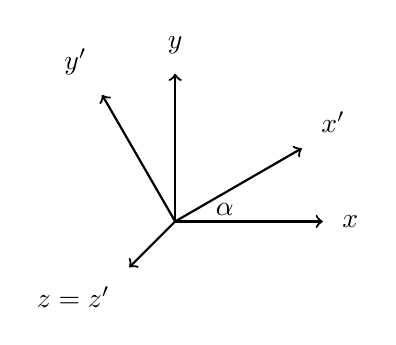
\begin{tikzpicture}
        \tikzstyle{axis} = [thick, ->]
        \node (x) at (2, 0) {};
        \node (y) at (0, 2) {};
        \node (z) at (-0.707, -0.707) {};
        \node (x') at (1.732, 1) {};
        \node (y') at (-1, 1.732) {};
        \draw[axis] (0, 0) -- (x);
        \draw[axis] (0, 0) -- (y);
        \draw[axis] (0, 0) -- (z);
        \node[right] at (x) {\(x\)};
        \node[above] at (y) {\(y\)};
        \node[below left] at (z) {\(z = z'\)};
        \draw[axis] (0, 0) -- (x');
        \draw[axis] (0, 0) -- (y');
        \node[above right] at (x') {\(x'\)};
        \node[above left] at (y') {\(y'\)};
        \centerarc[](0, 0)(0:30:0.5);
        \node at (0.63, 0.15) {\(\alpha\)};
    \end{tikzpicture}
    \caption{A passive rotation about the \(z\)-axis through an angle \(\alpha\).}
    \label{fig:rotation about z axis}
\end{figure}
It can be seen from the geometry that
\begin{align*}
    \vv{e'_x}\cdot\ve{x} &= \cos\alpha,\\
    \vv{e'_x}\cdot\ve{y} &= \cos\left(\frac{\pi}{2} - \alpha\right) = \sin\alpha,\\
    \vv{e'_y}\cdot\ve{x} &= \cos\left(\frac{\pi}{2} + \alpha\right) = -\sin\alpha,\\
    \vv{e'_y}\cdot\ve{y} &= \cos\alpha,
\end{align*}
etc. and we see that a rotation through angle \(\alpha\) about the \(z\) axis has the rotation matrix
\[
L_z(\alpha) =
\begin{pmatrix}
    \cos\alpha & \sin\alpha & 0\\
    -\sin\alpha & \cos\alpha & 0\\
    0 & 0 & 1
\end{pmatrix}
.
\]
Similarly it can be shown that a rotation by angle \(\beta\) about the \(x\) axis and a rotation by angle \(\gamma\) about the \(y\) axis have the following rotation matrices:
\[
L_x(\beta) = 
\begin{pmatrix}
    1 & 0 & 0\\
    0 & \cos\beta & \sin\beta\\
    0 & -\sin\beta & \cos\beta
\end{pmatrix}
,\qquad\text{and}\qquad L_y(\gamma) =
\begin{pmatrix}
    \cos\gamma & 0 & -\sin\gamma\\
    0 & 1 & 0\\
    \sin\gamma & 0 & \cos\gamma
\end{pmatrix}
.
\]
Since \(L_z(\alpha)\) represents a rotation we expect that its inverse is \(L_z^{-1}(\alpha) = L_z(-\alpha)\), and indeed this is the case.
By inspection using the fact that \(\sin\) is odd so \(\sin(-\alpha) = -\sin(\alpha)\) we can show that \(L_z(\alpha)\) is an orthogonal matrix.
This can be shown for a more general rotation matrix, \(L = (l_{ij})\), using the fact that the length of a vector is invariant under rotation of the basis so \(a^2 = \vv{a}\cdot\vv{a}\) should be the same before and after a rotation.
Before a rotation we have \(a^2 = a_ia_i = \delta_{ij} a_ia_j\).
After a rotation each component is transformed so we have \(a^2 = a'_ka'_k = (l_{ki}a_i)(l_{kj}a_j) = (l_{ki}l_{kj})a_ia_j\) so for \(a^2\) to be invariant we require \(l_{ki}l_{kj} = \delta_{ij}\).
Thus \((L\trans)_{ik}L_{kj} = (L\trans L)_{ij} = \delta_{ij}\) and so \(L\trans L = I\) meaning that \(L\in\orthogonalGroup(3)\).

We can also consider how the basis vectors, \(\{\ve{i}\}\), transform to the new basis vectors, \(\{\vv{e'_i}\}\).
Since a vector is not changed by a passive transform we have \(a'_i\vv{e'_i} = a_j\ve{j}\).
Inserting the transformation rule for \(a'_{i}\) we have \(l_{ij}a_i\vv{e'_i} = a_j\ve{j}\) which must hold for all vectors, \(\vv{a}\in\reals^3\) and therefore must hold for all \(a_i\in\reals\).
For this to be the case we must have \(l_{ij}\vv{e'_i} = \ve{j}\).
Multiplying through by \(l_{kj}\) this becomes \(l_{kj}l_{ij}\vv{e'_i} = l_{kj}\ve{j}\).
Now noting that \(l_{kj}l_{ij} = L_{kj}(L\trans)_{ji} = (LL\trans)_{ki} = \delta_{ki}\) we have \(\delta_{ki}\vv{e'_i} = \ve{e'_k} = l_{kj}\ve{j}\) which gives us the transformation rule for the basis vectors:
\[\vv{e'_i} = l_{ij}\ve{j}.\]

\begin{definition}{Proper and improper transformations}{}
    A transformation is called \define{proper} (or \define{improper}) if it preserves (or changes) the parity (i.e. left or right handed) of the system.
\end{definition}
A pure rotation is a proper transformation as a rotation of a right handed system will again be right handed.
An improper rotation also inverts the parity of the coordinate system.
A proper transformation will have a positive determinant whereas an improper rotation will have a negative determinant.
An improper rotation can be written as a proper rotation as well as a reflection in the origin.
\begin{notation*}{}
    The special orthogonal group, or rotation group, is the set of all proper rotations about the origin.
    It is denoted
    \[\specialOrthogonalGroup(n) = \{A\in\orthogonalGroup(n)\mid \det A = 1\} \subseteq \orthogonalGroup(n) \subseteq \generalLinearGroup(n) \subseteq \nxmMatrices{n}{n}{\reals}.\]
\end{notation*}

\subsection{Composition of Rotations}
Consider three bases, \(\{\ve{i}\}\), \(\{\vv{e'_i}\}\), and \(\{\vv{e''_i}\}\), related by \(\vv{e'_i} = l^{(1)}_{ij}\ve{j}\) and \(\vv{e''_i} = l^{(2)}_{ij}\vv{e'_j}\).
Then \(\vv{e''_i} = l_{ij}\vv{e'i} = l^{(2)}_{ij}l^{(1)}_{jk}\ve{k} = (L^{(2)}L^{(1)})_{ik}\ve{k}\).
The order is important.
In general rotation \(A\) and then rotation \(B\) is not the same as rotation \(B\) then rotation \(A\).
This is reflected by the non-commutativity of matrix multiplication.
The first transformation applied must be applied first and so is directly next to the object being transformed.

Any rotation about some arbitrary axis can be decomposed into three rotations around the Cartesian axis, first a rotation around the \(z\)-axis by angle \(\alpha\), then a rotation around the \(y'\)-axis by angle \(\beta\), then a rotation around the \(z''\)-axis by angle \(\gamma\).
These three angles are called the Euler angles and they encode the rotation matrix
\begin{align*}
    L(\alpha, \beta, \gamma) &= L_{z''}(\gamma)L_{y'}(\beta)L_{z}(\alpha)\\
    &=
    \begin{pmatrix}
        \cos\gamma & \sin\gamma & 0\\
        -\sin\gamma & \cos\gamma & 0\\
        0 & 0 & 1
    \end{pmatrix}
    \begin{pmatrix}
        \cos\beta & 0 & -\sin\beta\\
        0 & 1 & 0\\
        \sin\beta & 0 & \cos\beta
    \end{pmatrix}
    \begin{pmatrix}
        \cos\alpha & \sin\alpha & 0\\
        -\sin\alpha & \cos\alpha & 0\\
        0 & 0 & 1
    \end{pmatrix}
    \\
    &=
    \begin{pmatrix}
        \cos\beta\cos\alpha\cos\gamma - \sin\alpha\sin\gamma & \cos\beta\sin\alpha\cos\gamma + \cos\alpha\sin\gamma & -\sin\beta\cos\gamma\\
        -\cos\beta\cos\alpha\sin\gamma - \sin\alpha\cos\gamma & -\cos\beta\sin\alpha\sin\gamma + \cos\alpha\cos\gamma & \sin\beta\sin\gamma\\
        \sin\beta\cos\alpha & \sin\beta\sin\alpha & \cos\beta
    \end{pmatrix}
    .
\end{align*}

\section{Active Rotations}
\subsection{General Rotations}
An active rotation keeps the basis fixed and rotates the vector.
In this section we will derive the transformation matrix for a rotation about the unit vector, \(\vh{n}\), by an angle \(\vartheta\) of a vector \(\vv{x}\).
\begin{figure}[ht]
    \centering
    \tikzsetnextfilename{active-rotation}
    \begin{tikzpicture}
        \tikzstyle{line} = [thick]
        \node[inner sep=0cm] (O) at (0, 0) {};
        \node[inner sep=0cm] (S) at (0, 3) {};
        \node[inner sep=0cm] (P) at (2, 3) {};
        \node[inner sep=0cm] (Q) at (1.6, 3.4) {};
        \node[below] at (O) {\(O\)};
        \node[right] at (P) {\(P\)};
        \node[above right] at (Q) {\(Q\)};
        \node[left] at (S) {\(S\)};
        \draw[line] (O) -- (P);
        \draw[line] (O) -- ($(S) + (0, 1)$);
        \draw[line] (S) -- (P);
        \draw[line, dashed]  (S) -- (Q);
        \draw[line, dashed] (O) -- (Q);
        \draw[line, ->] (O) -- ($(O)!.5!(P)$) node[right] {\(\vv{x}\)};
        \draw[line, ->] ($(O)!.499!(Q)$) -- ($(O)!.501!(Q)$) node[left] {\(\vv{y}\)};
        \draw[line, ->] (O) -- ($(O)!0.3!(S)$) node[left] {\(\vh{n}\)};
        \begin{scope}
            \clip (S) -- ($(P) + (P) - (S)$) -- ($(Q) + (Q) - (S)$) -- (S);
            \draw[line] (P) arc (30:100:1.3);
            \draw (S) circle[radius=0.75cm];
        \end{scope}
        \node at ($(S) + (0.4, 0.3)$) {\small\(\vartheta\)};
        
        \node[inner sep=0cm] (S2) at (4, 1) {};
        \node[inner sep=0cm] (P2) at ($(S2) + (2, 0)$) {};
        \node[inner sep=0cm] (Q2) at ($(S2) + ({2 * cos(30)}, {2 * sin(30)})$) {};
        \node[inner sep=0cm] (nx) at ($(S2) + (0, 1)$) {};
        \node[inner sep=0cm] (T) at ($(S2)!(Q2)!(P2)$) {};
        \node at (S2) {\large\(\odot\)};
        \node[left] at ($(S2) - (0.1, 0)$) {\(\vh{n}\)};
        \draw[line] (S2) -- (P2);
        \draw[line] (S2) -- (Q2);
        \draw[line, ->] (S2) -- (nx) node[above] {\(\vh{n} \times \vv{x}\)};
        \draw[line, dashed] (Q2) -- (T);
        \node[below] at ($(S2) - (0, 0.1)$) {\(S\)};
        \node[right] at (P2) {\(P\)};
        \node[above] at (Q2) {\(Q\)};
        \node[below] at (T) {\(T\)};
        \draw[line] (P2) arc (0:30:2);
        \draw ($(S2)!.2!(P2)$) arc (0:30:.4);
        \node at ($(S2) + (0.6, 0.15)$) {\small\(\vartheta\)};
    \end{tikzpicture}
    \caption{An active rotation of vector \(\vv{x}\) into vector \(\vv{y}\). Shown on the left is a view from the side. Shown on the right is a view from above.}
    \label{fig:active rotation}
\end{figure}
Consider figure~\ref{fig:active rotation}.
This shows the vector \(\vv{x}\) which is the position vector of the point \(P\).
We consider a rotation about \(\vh{n}\) by angle \(\vartheta\) to take the point \(P\) to the point \(Q\) which has position vector \(\vv{y}\).
We also define \(S\) as the projection of \(P\) or \(Q\) onto \(\vh{n}\).
Then \(\overrightarrow{OS}\) is the component of \(\vv{x}\) in the \(\vh{n}\) direction, which is given by \(\overrightarrow{OS} = (\vv{x}\cdot\vh{n})\vh{n}\).
Further let \(T\) be the projection of \(Q\) onto the vector \(\overrightarrow{SP}\).
This means that \(\overrightarrow{TQ}\) is parallel to \(\vh{n}\times\vv{x}\).
We can see that
\begin{align*}
    \vv{y} &= \overrightarrow{OS} + \overrightarrow{ST} + \overrightarrow{TQ}\\
    &= (\vv{x}\cdot\vh{n})\vh{n} + \underbrace{SQ\cos\vartheta}_{\abs{\overrightarrow{ST}}} \underbrace{\frac{\vv{x} - (\vv{x}\cdot\vh{n})\vh{n}}{SP}}_{\widehat{\overrightarrow{SP}}} + \underbrace{SQ\sin\vartheta}_{\abs{\overrightarrow{TQ}}} \underbrace{\frac{\vh{n}\times\vv{x}}{\abs{\vh{n}\times\vv{x}}}}_{\widehat{\overrightarrow{TQ}}}\\
    &= (\vv{x}\cdot\vh{n})\vh{n} + \cos(\vartheta)(\vv{x} - (\vv{x}\cdot\vh{n})\vh{n}) + \sin(\vartheta) (\vh{n}\times\vv{x}).
\end{align*}
Here we have used the fact that \(SP = SQ\) since the distance between the axis of rotation and a rotated point is maintained by definition in a rotation.
Also \(\abs{\vh{n}\times\vv{x}} = SP = SQ\).
The result that we end up with is
\[\vv{y} = \vv{x} \cos\vartheta + (1 - \cos\vartheta) (\vh{n}\cdot\vv{x})\vh{n} + (\vh{n}\times\vv{x})\sin\vartheta.\]
This can be written in index notation as
\[y_i = x_i\cos\vartheta + (1 - \cos\vartheta) n_jx_jn_i + \varepsilon_{ikj}n_kx_j\sin\vartheta\]
note the unusual ordering, \((i, k, j)\), for the Levi--Civita symbol which is to match conventions later.
We can rewrite this as
\[y_i = R_{ij}(\vartheta, \vh{n}) = x_j\]
where 
\[R_{ij}(\vartheta, \vh{n}) = \delta_{ij} \cos\vartheta + (1 - \cos\vartheta)n_in_j - \varepsilon_{ijk}n_k\sin\vartheta.\]
\begin{definition}{Rotation matrix}{}
    An active rotation of angle \(\vartheta\) about the axis \(\vh{n}\) can be represented by the \define{rotation matrix} \(R\in\nxmMatrices{3}{3}{\reals}\) with components
    \[R_{ij} = \delta_{ij} \cos\vartheta + (1 - \cos\vartheta)n_in_j - \varepsilon_{ijk}n_k\sin\vartheta.\]
\end{definition}
\begin{theorem}{Rotation matrices are orthogonal}{}
    Rotation matrices are orthogonal.
\end{theorem}
% TODO : Complete proof after workshop
%    \begin{proof}[Proof 1]
%        Let \(R\) be a rotation matrix.
%        Then
%        \begin{align*}
%            [RR\trans]_{ij} &= R_{ik}[R\trans]_{kj}\\
%            &= R_{ik}R_{jk}\\
%            &= [\delta_{ik}\cos\vartheta + (1 - \cos\vartheta)n_in_k - \varepsilon_{ikl}n_l\sin\vartheta] [\delta_{jk}\cos\vartheta + (1 - \cos\vartheta)n_jn_k - \varepsilon_{jkm}n_m\sin\vartheta]\\
%            &= \delta_{ik}\delta_{jk}\cos^2\vartheta + \delta_{ik}(1 - \cos\vartheta)n_jn_k - \delta_{ik}\varepsilon_{jkm}n_m\sin\vartheta\\
%            &\qquad + (1 - \cos\vartheta)n_in_k\delta_{jk}\cos\vartheta + (1 - \cos\vartheta)^2n_in_kn_jn_k - (1 - \cos\vartheta)n_in_k\varepsilon_{jkm}n_m\sin\vartheta\\
%            &\qquad - \varepsilon_{ikl}\delta_{jk}n_l\sin\vartheta \cos\vartheta - \varepsilon_{ikl}n_l\sin\vartheta(1 - \cos\vartheta)n_jn_k + \varepsilon_{ikl}\varepsilon_{jkm}n_ln_m\sin^2\vartheta\\
%            &= \delta_{ij}\cos^2\vartheta + (1 - \cos\vartheta)n_jn_i - \varepsilon_{jim}n_m\sin\vartheta\\
%            &\qquad + n_in_j(1 - \cos\vartheta)\cos\vartheta + (1 - \cos\vartheta)n_in_j - \varepsilon_{jkm}n_in_kn_m\sin\vartheta\\
%            &\qquad + \varepsilon_{ijl}n_l\sin\vartheta\cos\vartheta - \varepsilon_{ikl}n_l\sin\vartheta(1 - \cos\vartheta)n_jn_k + 
%        \end{align*}
%    \end{proof}
\begin{proof}[Proof 2]
    A rotation preserves lengths.
    Since we can define the length of a vector, \(\vv{x}\), to be \(\sqrt{\vv{x}\cdot\vv{x}}\) this means a rotation preserves inner products.
    Therefore by corollary~\ref{cor:orthogonal transformations preserve inner products} rotations are orthogonal transformations.
\end{proof}

\begin{lemma}{Rotation matrix properties}{}
    If \(R\) is a rotation matrix then
    \[\Tr R = 1 + 2\cos\vartheta, \qquad\text{and}\qquad n_k\sin\vartheta = -\frac{1}{2}\varepsilon_{ijk}R_{ij}.\]
\end{lemma}
\begin{proof}
    Let \(R\) be a rotation matrix.
    \[\delta_{ij}R_{ij} = R_{ii} = \Tr R\]
    Also
    \begin{align*}
        \delta_{ij}R_{ij} &= \delta_{ij}[\delta_{ij} \cos\vartheta + (1 - \cos\vartheta)n_in_j - \varepsilon_{ijk}n_k\sin\vartheta]\\
        &= \delta_{ii}\cos\vartheta + (1 - \cos\vartheta)\underbrace{n_in_i}_{\mathclap{=\vh{n}\cdot\vh{n} = 1}} - \underbrace{\delta_{ij}\varepsilon_{ijk}}_{=\varepsilon_{iik} = 0}n_k\sin\vartheta\\
        &= 3\cos\vartheta + 1 - \cos\vartheta\\
        &= 1 + 2\cos\vartheta.
    \end{align*}
    Now consider
    \begin{align*}
        \varepsilon_{ijk}R_{ij} &= \varepsilon_{ijk}[\delta_{ij} \cos\vartheta + (1 - \cos\vartheta)n_in_j - \varepsilon_{ijl}n_l\sin\vartheta]\\
        &= \underbrace{\varepsilon_{ijk}\delta_{ij}}_{=\varepsilon_{iik} = 0}\cos\vartheta + (1 - \cos\vartheta)\underbrace{\varepsilon_{ijk}n_in_j}_{(\vh{n}\times\vh{n})_k = 0} - \underbrace{\varepsilon_{ijk}\varepsilon_{ijl}}_{=2\delta_{lk}} n_l\sin\vartheta\\
        &= -2\delta_{lk}n_l\sin\vartheta\\
        &= -2n_k\sin\vartheta.
    \end{align*}
    Rearranging we have
    \[-\frac{1}{2}\varepsilon_{ijk}R_{ij} = n_k\sin\vartheta.\]
\end{proof}
We can use these two identities to find \(\vh{n}\) and \(\vartheta\) given a rotation matrix, \(R\).

As with passive transformation the product of two rotations is a rotation and the order matters.
For example the vector given by rotating \(\vv{x}\) by rotation \(R\) and then rotation \(S\) is \(SR\vv{x}\) which is not necessarily equal to \(RS\vv{x}\).

\subsection{Rotational Symmetry}
If we consider an infinitesimal rotation by \(\delta\vartheta\) and we allow \(\delta\vartheta \to 0\) then we can use the Taylor series,
\[\sin(\delta\vartheta) = \delta\vartheta + \order{\delta\vartheta^3} \qquad\text{and}\qquad \cos(\delta\vartheta) = 1 + \order{\delta\vartheta^2},\]
to write
\[R_{ij} = \delta_{ij} - \varepsilon_{ijk}n_k\delta\vartheta.\]
Going back to vectors from components we have
\[y_i = R_{ij}x_j = \delta_{ij}x_j - \varepsilon_{ijk}n_kx_j\delta\vartheta = x_i + \varepsilon_{ikj}n_kx_j\delta\vartheta\]
which gives
\[\vv{y} = R\vv{x} = \vv{x} + (\vh{n}\times\vv{x})\delta\vartheta.\]

We can write the component form of the infinitesimal rotation matrices as
\[R_{ij} = \delta_{ij} - \varepsilon_{ijk}n_k\delta\vartheta = \delta_{ij} - in_k(T_k)_{ij}\delta\vartheta\]
Where we have defined three matrices \(T_k\) with components \((T_k)_{ij} = -i\varepsilon_{ijk}\).
These matrices in full are
\[
T_1 = i
\begin{pmatrix}
    0 & 0 & 0\\
    0 & 0 & -1\\
    0 & 1 & 0
\end{pmatrix}
, \qquad T_2 = i
\begin{pmatrix}
    0 & 0 & 1\\
    0 & 0 & 0\\
    -1 & 0 & 0
\end{pmatrix}
, \qquad T_3 = i
\begin{pmatrix}
    0 & -1 & 0\\
    1 & 0 & 0\\
    0 & 0 & 0
\end{pmatrix}
.
\]
We say that the matrices \(T_i\) are the generators of rotations in the sense that any infinitesimal rotation matrix can be made from \(T_i\) and any rotation can be made from an infinite number of infinitesimal rotation matrices.
We will see how shortly.

If we commit a small abuse of notation and define a `vector' \(\vv{T} = (T_1, T_2, T_3)\) then we can write \(R\) as
\[R(\delta\vartheta, \vh{n}) = \ident - i\delta\vartheta (\vh{n}\cdot\vv{T}).\]
Note that
\[\vh{n}\cdot\vv{T} = n_1T_1 + n_2T_2 + n_3T_3 \in\nxmMatrices{3}{3}{\complex}.\]

\begin{definition}{Commutator}{}
    Let \(A, B\in\nxmMatrices{n}{n}{\complex}\) then we define the \define{commutator}, 
    \[[\cdot, \cdot]\colon \nxmMatrices{n}{n}{\complex}\times \nxmMatrices{n}{n}{\complex} \to \nxmMatrices{n}{n}{\complex}\]
    as
    \[[A, B] = AB - BA.\]
    This measures the degree to which \(A\) and \(B\) fail to commute.
\end{definition}
It can be shown that
\[[T_i, T_j] = i\varepsilon_{ijk}T_k\]
which should be familiar from quantum mechanics as the commutation relation for angular momentum components (possibly with an extra factor of \(\hbar\)).
There is a reason for this.
Since \(T_i\) are the generators of rotations they lead to angular momentum in the same way that the generator of translations leads to linear momentum.

The commutation relations between the generators form part of the Lie\footnote{pronounced `lee'.} algebra, \(\lieAlgebra{so}(3)\).
This is the Lie algebra of the Lie group \(\specialOrthogonalGroup(3)\).
What this means is that the elements of \(\lieAlgebra{so}(3)\) generate \(\specialOrthogonalGroup(3)\).
The elements of \(\lieAlgebra{so}(3)\) are the are the commutator of linear combinations of \(T_i\), for example 
\[[T_1 + 2T_2, T_3] = [T_1, T_3] + 2[T_2, T_3] = -iT_2 + 2iT_1 \in \lieAlgebra{so}(3).\]
We say that \(T_i\) generate \(\lieAlgebra{so}(3)\).
To construct a finite rotation of angle \(\vartheta\) about \(\vh{n}\) we consider \(N\) infinitesimal translations each taking us \(\delta\vartheta = \vartheta/N\) and then take \(N\to\infty\).
So the rotation matrix is
\begin{align*}
    R(\vartheta, \vh{n}) &= \lim_{N\to\infty} [R(\delta\vartheta, \vh{n})]^N\\
    &= \lim_{N\to\infty} \left[\ident - i \frac{\vartheta}N{}\vh{n}\cdot\vv{T}\right]^N\\
    &= \exp\left[-i\vartheta\vh{n}\cdot\vv{T}\right].
\end{align*}
Here we have used
\[e^x = \lim_{N\to\infty}\left[1 + \frac{x}{N}\right]^N\]
and assumed that this holds for exponentials containing matrices.
Recall also that functions of matrices are defined through their power series and therefore
\[e^A = 1 + A + \frac{1}{2!}A^2 + \frac{1}{3!}A^3 + \dotsc.\]
See appendix~\ref{app:Lie algebras} for more detail on Lie algebras.


\section{Tensors}
\subsection{Reflections}
We will start this section with a definition and explain it after:
\begin{definition}{Reflection and Inversion}{}
    The \define{reflection} of a vector, \(\vv{x}\), in a plane with surface normal \(\vh{n}\) is given by
    \[\vv{y} = \vv{x} - 2(\vv{x}\cdot\vh{n})\vh{n}\]
    or
    \[y_i = \sigma_{ij}x_j, \qquad\text{where}\qquad \sigma_{ij} = \delta_{ij} - 2n_in_j.\]
    An \define{inversion} of a vector, which is a reflection through the origin, is given by
    \[\vv{y} = -\vv{x}\]
    or
    \[y_i = P_{ij}x_j, \qquad\text{where}\qquad P_{ij} = -\delta_{ij}.\]
    \(P_{ij}\) is called the \define{parity operator}.
\end{definition}
Consider the setup drawn in figure~\ref{fig:reflected vector}.
From this it should be clear that \(\vv{x} - (\vv{x}\cdot\vh{n})\vh{n}\) is the projection of \(\vv{x}\) onto the plane.
Subtracting \((\vv{x}\cdot\vh{n})\vh{n}\) again gives us a vector the same distance below the plane again.
\begin{figure}[ht]
    \centering
    \tikzsetnextfilename{reflection}
    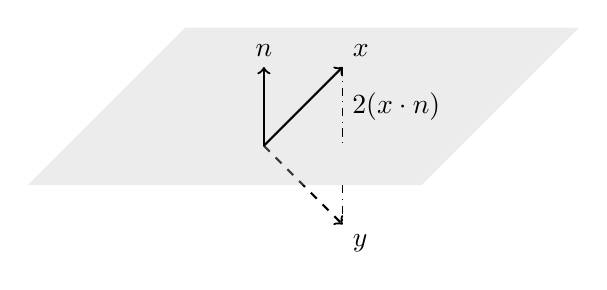
\begin{tikzpicture}
        \draw[thick, dashed, ->] (1, 0) -- (2, -1) node[below right] {\(\vv{y}\)};
        \fill[fill=lightgray, opacity=0.3] (-2, -0.5) -- (0, 1.5) -- (5, 1.5) -- (3, -0.5) -- cycle;
        \draw[thick, ->] (1, 0) -- (1, 1) node[above] {\(\vh{n}\)};
        \draw[thick, ->] (1, 0) -- (2, 1) node[above right] {\(\vv{x}\)};
        \draw[dash dot] (2, 1) -- (2, 0) node[midway, right] {\(2(\vv{x}\cdot\vh{n})\)};
        \draw[dash dot] (2, -0.5) -- (2, -1);
    \end{tikzpicture}
    \caption{A vector, \(\vv{x}\), and its reflection, \(\vv{y}\), in the plane with surface normal \(\vh{n}\).}
    \label{fig:reflected vector}
\end{figure}

A reflection in the origin simply negates each component which is clearly the effect of the parity operator as described above.
Further we can see this as a reflection where the vector being reflected is also the surface normal.
Therefore the inverted vector is
\[\vv{y} = \vv{x} - 2(\vv{x}\cdot\vh{x})\vh{x} = \vv{x} - 2x\vh{x} = \vv{x} - 2\vv{x} = -\vv{x}.\]

Reflections are self inverses, that is \(P^2 = \sigma^2 = I\).
They are also improper transformations, i.e. \(\det P = \det\sigma = -1\)\footnote{Inversion is only an improper transformation in an odd number of dimensions. In even dimensions all the negatives cancel to give a determinant of \(+1\)}.
This means that reflections and inversions are included in \(\orthogonalGroup(n)\).
In fact reflections generate \(\orthogonalGroup(n)\), by this we mean that any element of \(\orthogonalGroup(n)\), including rotations, can be made of some number of reflections.
Rotations, as proper transformations, must be composed of an even number of reflections.

\subsection{Projection Operators}
\begin{definition}{Projection Operators}{}
    \(P_{\vv{u}}\) is a \define{parallel projection operator} onto a vector \(\vv{u}\) if
    \[P_{\vv{u}}\vv{u} = \vv{u}, \qquad\text{and}\qquad P_{\vv{u}}\vv{v} = \vv{0}\]
    where \(\vv{v}\) is orthogonal to \(\vv{u}\).
    \(Q_{\vv{u}}\) is an \define{orthogonal projection operator} to \(\vv{u}\) if
    \[Q_{\vv{u}}\vv{u} = \vv{0}, \qquad\text{and}\qquad Q_{\vv{u}}\vv{v} = \vv{v}\]
    where, again, \(\vv{v}\) is orthogonal to \(\vv{u}\).
\end{definition}
Let \(\vv{u}\) and \(\vv{v}\) be orthogonal vectors.
Then
\begin{align*}
    (I - P_{\vv{u}})\vv{u} &= I\vv{u} - P_{\vv{u}}\vv{u} = \vv{u} - \vv{u} = \vv{0},\\
    (I - P_{\vv{u}})\vv{v} &= I\vv{v} - P_{\vv{u}}\vv{v} = \vv{v} - \vv{0} = \vv{v}.
\end{align*}
We see that \(Q_{\vv{u}} = I - P_{\vv{u}}\).
Suitable operators are
\[P_{\vv{u}ij} = \frac{u_iu_j}{u^2}, \qquad\text{and}\qquad Q_{\vv{u}ij} = \delta_{ij} - \frac{u_iu_j}{u^2}.\]
\begin{lemma}{Uniqueness of projection operators}{}
    The projection operators for a given vector, \(\vv{u}\in\reals^3\), are unique.
\end{lemma}
\begin{proof}
    Suppose \(P_{\vv{u}}\) and \(T_{\vv{u}}\) are both parallel projection operators for \(\vv{u}\).
    Let \(\vv{u}\) and \(\vv{v}\) be orthogonal.
    Then \(\{\vv{u}, \vv{v}, \vv{u}\times\vv{v}\}\) spans \(\reals^3\) and are all mutually orthogonal.
    Thus any vector, \(\vv{w}\in\reals^3\), can be written as a linear combination:
    \[\vv{w} = \mu\vv{u} + \nu\vv{v} + \lambda(\vv{u}\times\vv{v}).\]
    Consider now the operator \(P_{\vv{u}} - T_{\vv{u}}\):
    \begin{align*}
        (P_{\vv{u}} - T_{\vv{u}})\vv{w} &= (P_{\vv{u}} - T_{\vv{u}}) [\mu\vv{u} + \nu\vv{v} + \lambda(\vv{u}\times\vv{v})]\\
        &= \mu P_{\vv{u}}\vv{u} + \nu P_{\vv{u}}\vv{v} + \lambda P_{\vv{u}}(\vv{u}\times\vv{v}) - \mu T_{\vv{u}}\vv{u} - \nu T_{\vv{u}}\vv{v} - \lambda T_{\vv{u}}(\vv{u}\times\vv{v})\\
        &= \mu\vv{u} - \mu\vv{u}\\
        &= \vv{0}
    \end{align*}
    so \(P_{\vv{u}}\vv{w} = T_{\vv{u}}\vv{w}\) for all \(\vv{w}\in\reals^3\) which means \(P_{\vv{u}} = T_{\vv{u}}\).
    
    Suppose now that \(Q_{\vv{u}}\) and \(S_{\vv{u}}\) are orthogonal projection operators for \(\vv{u}\).
    Then
    \begin{align*}
        (Q_{\vv{u}} - S_{\vv{u}})\vv{w} &= (Q_{\vv{u}} - S_{\vv{u}}) [\mu\vv{u} + \nu\vv{v} + \lambda(\vv{u}\times\vv{v})]\\
        &= \mu Q_{\vv{u}}\vv{u} + \nu Q_{\vv{u}}\vv{v} + \lambda Q_{\vv{u}}(\vv{u}\times\vv{v}) - \mu S_{\vv{u}}\vv{u} - \nu S_{\vv{u}}\vv{v} - \lambda S_{\vv{u}}(\vv{u}\times\vv{v})\\
        &= \nu\vv{v} + \lambda(\vv{u}\times\vv{v}) - \nu\vv{v} - \lambda(\vv{u}\times\vv{v})\\
        &= \vv{0}
    \end{align*}
    Hence \(Q_{\vv{u}} = S_{\vv{u}}\).
\end{proof}
Note that projection operators are \emph{not} orthogonal.
For example if \(\{\ve{i}\}\) is an orthonormal basis then \(\ve{1} + \ve{2}\) has length \(\sqrt{2}\) and \(P_{\ve{1}}(\ve{1} + \ve{2}) = \ve{1}\) has length \(1\) so \(P_{\ve{1}}\) doesn't preserve inner products so is not orthogonal.

\subsection{Active and Passive Transformations}
Recall that an active transformation involves changing the vector and a passive rotation involves changing the basis.

Consider the case when the basis, \(\{\ve{i}\}\) is transformed to \(\{\vv{e'_i}\}\) such that \(\vv{x} = x_i\ve{i} = x'_i\vv{e'_i}\), with \(x'_i = l_{ij}x_j\).
This is a passive transformation but we can define a rotation matrix, \(R_{ij} = l_{ij}\) and consider the vector \(\vv{y} = R\vv{x}\) with components \(y_i = R_{ij}x_j\).
Clearly \(y_i = l_P={ij} = x'_j\).
If we consider an active rotation about the \(z\)-axis then we have
\begin{align*}
    R_{ij}(\vartheta, \ve{3}) &= \delta_{ij} + (1 - \cos\vartheta)\delta_{i3}\delta_{j3} - \varepsilon_{ijk}\delta_{k3}\sin\vartheta,\\
    R &= 
    \begin{pmatrix}
        \cos\vartheta & -\sin\vartheta & 0\\
        \sin\vartheta & \cos\vartheta & 0\\
        0 & 0 & 1
    \end{pmatrix}
    .
\end{align*}
Here we have used that \(\ve{3} = n_i\) so \(n_i = \delta_{i3}\).
This matrix corresponds to an active transformation through the angle \(\vartheta\).

If instead we consider how the basis changes then we can readily see that
\begin{align*}
    \vv{e'_1} &= \cos\vartheta\ve{1} - \sin\vartheta\ve{2}\\
    \vv{e'_2} &= \sin\vartheta\ve{1} + \cos\vartheta\ve{2}\\
    \vv{e'_3} &= \ve{3}.
\end{align*}
This is a passive rotation through angle \(-\vartheta\).

In general an active rotation of \(\vv{x}\) is the same as a passive rotation of basis vectors through an equal and opposite angle.
The only thing that changes is what we are aiming to describe.
An active transformation may represent a point on a rigid body moving whereas a passive transformation may represent a frame of reference rotating.

\subsection{Tensors}
\subsubsection{Vectors}
We have seen that under a rotation of the basis given by \(L\in\specialOrthogonalGroup(3)\) all vectors, \(\vv{a}\in\reals^3\), transform as
\[a'_i = l_{ij}a_j.\]
We now turn this on its head to give us a new definition of a vector:
\begin{definition}{Vector, tensor definition}{}
    A \define{vector}, \(\vv{a}\in\reals^d\), is an entity with \(d\) components, \(a_i\), with respect to any basis.
    The components transform under a rotation, \(L\in\specialOrthogonalGroup(d)\), as
    \[a'_i = l_{ij}a_j.\]
\end{definition}

\subsubsection{Tensor Motivation}
Consider two vectors \(\vv{a}, \vv{b}\in\reals^d\).
The object \(a_ib_j\) has \(d^2\) components.
We want this object to transform in a way that means \((a_ib_j)' = a'_ib_j'\).
If this is the case then
\[(a_ib_j)' = a'_ib'_j = l_{i\alpha}a_\alpha l_{j\beta}b_{\beta} = (l_{i\alpha}l_{j\beta})(a_\alpha b_\beta).\]

\subsubsection{Tensor Definitions}
\begin{definition}{Rank 2 tensor}{}
    A \define{rank 2 tensor}, \(T\), in \(d\) dimensions is an object with \(d^2\) components, \(T_{ij}\), with respect to any basis.
    The components transform under a rotation, \(L\in\specialOrthogonalGroup(d)\), as
    \[T'_{ij} = l_{i\alpha}l_{j\beta}T_{\alpha\beta}.\]
\end{definition}
Notice from this definition that \(a_ib_j\) as defined in the last section is a rank 2 tensor but not all rank two tensor components can be written as a product of vector components.

We can generalise this definition to a rank \(n\) tensor:
\begin{definition}{Rank \(\bm{n}\) tensor}{}
    A \define{rank \(\mathdefine{n}\) tensor}, \(T\), in \(d\) dimensions is an object with \(d^n\) components, \(T_{i_1i_2\dotsm i_n}\), with respect to any basis.
    The components transform under a rotation, \(L\in\specialOrthogonalGroup(d)\), as
    \[T'_{i_1i_2\dotsm i_n} = l_{i_1\alpha_1}l_{i_2\alpha_2}\dotsm l_{i_n\alpha_n}T_{\alpha_1\alpha_2\dotsm\alpha_n}.\]
\end{definition}
The most common case for us will be \(d = 3\) where a rank \(n\) tensor is an object with \(3^n\) components, \(T_{i_1i_2\dotsm i_n}\), that transforms under a rotation, \(L\in\specialOrthogonalGroup(3)\), as
\[T'_{i_1i_2\dotsm i_n} = l_{i_1\alpha_1}l_{i_2\alpha_2}\dotsm l_{i_n\alpha_n}T_{\alpha_1\alpha_2\dotsm\alpha_n}.\]
Note the distinction between rank and dimension.
The rank is the number of indices whereas the dimension gives the possible values that each index can take, in general \(i = 1, \dotsc, d\) for a \(d\)-dimensional tensor.

From these definitions we can make two immediate observations:
\begin{itemize}
    \item A vector is a rank 1 tensor, i.e. \(a_i = l_{i\alpha}a_{\alpha}\).
    \item A scalar is a rank 2 tensor, i.e. \(\varphi = \varphi'\).
\end{itemize}

While technically incorrect we will often say that \(T_{i_1i_2\dotsm i_n}\) is a rank \(n\) tensor when what we really mean is that \(T_{i_1i_2\dotsm i_n}\) are the components of a rank \(n\) tensor, \(T\).
In this course we make no distinction between covariant and contravariant indices.
As such we use only lower indices since we don't need to separate the two concepts.
Also since we are almost only interested in three dimensional Euclidean space we don't follow the normal convention where Greek indices run from 0 to 3 or 1 to 4 as is common when doing relativity.
As a final note for this section while all vectors are tensors not all matrices are tensors.
By this we mean that a matrix doesn't necessarily have an associated transformation law.
This is the same as saying that although a vector can be written as a tuple not all tuples are vectors.

\section{Properties of Tensors}
\subsection{Tensor Fields}
\begin{definition}{Tensor field}{}
    Let \(\mathcal{T}_n\) be the set of all rank \(n\) tensors.
    Then a \define{tensor field} is any function \(T\colon\reals^3 \to \mathcal{T}_n\).
    That is a tensor field assigns a tensor to every point in space.
\end{definition}
An example of a tensor field is the strain in a material which is a rank 2 tensor field with components \(E_{ij}(\vv{r})\).
Since at any particular point \(E_{ij}(\vv{r})\) are just the components of a tensor then \(E_{ij}\) transform as
\[E'_{ij}(\vv{r}) = l_{i\alpha}l_{j\beta}E_{\alpha\beta}(\vv{r}).\]
In the left hand side of this equation the components of \(\vv{r}\) are considered in the \(\{\vv{e'_i}\}\) basis whereas in the right hand side they are considered in the \(\{\ve{i}\}\) basis.
To emphasis this we often write \(E'_{ij}(x'_k) = l_{i\alpha}l_{j\beta}E_{\alpha\beta}(x_k)\).
Here \(x_k\) is shorthand for \((x_1, x_2, x_3)\) rather than meaning a specific coordinate.

\subsection{Dyadic Notation}
Dyadic notation is a notation sometimes used when working with tensors of rank \(n \le 2\).
\begin{notation*}{}
    In dyadic notation scalars and vectors are represented as we are used to.
    Normally this means that scalars are simply letters, such as \(a\) or \(\varphi\), and vectors are either bold or have an arrow or under line, such as \(\vv{v}\), \(\vec{v}\) or \(\underline{v}\).
    Rank 2 tensors are then notated in a similar way with an extra arrow, underline or double headed arrow.
    For example \(\vec{\vec{T}}\), \(\overset{\tiny\leftrightarrow}{T}\) or \(\underline{\underline{T}}\).
\end{notation*}
Dyadic notation is often less clear on meaning and therefore we won't use it here (apart from for vectors).
We provide a short dictionary here for translation into index notation.
\[
\begin{array}{ccc}\hline
    \text{Dyadic} &  & \text{Index}\\\hline
    \vec{a} & \longleftrightarrow & a_i\\
    \vec{a} \cdot \vec{b} & \longleftrightarrow & a_ib_i\\
    \overset{\tiny\leftrightarrow}{T} & \longleftrightarrow & T_{ij}~\text{or}~t_{ij}\\
    \vec{a}\overset{\tiny\leftrightarrow}{T}\vec{b} & \longleftrightarrow & a_iT_{ij}b_j\\\hline
\end{array}
\]

\subsection{Consistency of the Tensor Definition}
Let \(\basis = \{\ve{i}\}\), \(\basis' = {\veprime\{i\}}\), and \(\basis'' = \vepprime\{i\}\) be bases related by \(\veprime{i} = l_{ij}\ve{j}\) and \(\vepprime{i} = m_{ij}\veprime{j}\) where \(L, M\in\specialOrthogonalGroup(3)\).
We know that \(\basis\) and \(\basis''\) are related by the transformation matrix \(N = ML\) so \(\vepprime{i} = n_{ij}\ve{j}\).
For the definition of the transformation of a tensor to be consistent we need multiple transformations chained together to give the same components as a single equivalent transformation.
We will show here that this is the case for a rank 2 tensor \(T\) which has components \(T_{ij}\) in \(\basis\), \(T'_{ij}\) in \(\basis'\) and \(T''_{ij}\) in \(\basis''\).
This demonstration generalises easily to any given \(n\).
\begin{align*}
    T''_{ij} &= m_{i\alpha} m_{j\beta} T'_{\alpha\beta}\\
    &= m_{i\alpha}m_{j\beta} (l_{\alpha r}l_{\beta s}T_{rs})\\
    &= (m_{i\alpha}l_{\alpha r})(m_{j\beta}l_{\beta s}) T_{rs}\\
    &= (ML)_{ir}(ML)_{js} T_{rs}\\
    &= n_{ir}n_{js}T_{rs}
\end{align*}
which is exactly the same result we would expect going directly from \(\basis\) to \(\basis''\).

\subsubsection{Properties of Cartesian Tensors}
In this section we will prove various results about tensors.
Most of these will be no surprise as they are simply generalisations of ideas we have met with vectors and matrices.
\begin{lemma}{Sum of tensors is a tensor}{sum of tensors is a tensor}
    If \(T\) and \(U\) are rank \(n\) tensors then the object \(V\) with components
    \[V_{\nindices{i}{n}} = T_{\nindices{i}{n}} + U_{\nindices{i}{n}}\]
    is also a tensor of rank \(n\).
\end{lemma}
\begin{proof}
    Let \(T\) and \(U\) be tensors of rank \(n\) with components \(T_\nindices{i}{n}\) and \(U_\nindices{i}{n}\) in \(\basis = \{\ve{i}\}\) and components \(T'_\nindices{i}{n}\) and \(U'_\nindices{i}{n}\) in basis \(\basis' = \{\veprime{i}\}\) where \(\veprime{i} = l_{ij}\ve{j}\).
    Let \(V\) have components \(V_\nindices{i}{n} = T_\nindices{i}{n} + U_\nindices{i}{n}\) which transform as
    \begin{align*}
        V'_{\nindices{i}{n}} &= T'_\nindices{i}{n} + U'_\nindices{i}{n}\\
        &= l_{i_1\alpha_1}l_{i_2\alpha_2} \dotsm l_{i_n\alpha_n} T_\nindices{\alpha}{n} + l_{i_1\alpha_1}l_{i_2\alpha_2} \dotsm l_{i_n\alpha_n} U_\nindices{\alpha}{n}\\
        &= l_{i_1\alpha_1}l_{i_2\alpha_2} \dotsm l_{i_n\alpha_n} (T_\nindices{\alpha}{n} + U_\nindices{\alpha}{n})\\
        &=l_{i_1\alpha_1}l_{i_2\alpha_2} \dotsm l_{i_n\alpha_n} V_\nindices{\alpha}{n}.
    \end{align*}
    So \(V\) follows the expected transformation laws and is a rank \(n\) tensor.
\end{proof}

\begin{lemma}{Product of tensors is a tensor}{product of tensors is tensor}
    If \(T\) is a rank \(n\) tensor and \(U\) is a rank \(m\) tensor then the object \(V\) with components
    \[V_{\nindices{i}{n}\nindices{j}{m}} = T_{\nindices{i}{n}}U_{\nindices{j}{m}}\]
    is a tensor of rank \(n + m\).
\end{lemma}
\begin{proof}
    Let \(T\) and \(U\) be tensors of rank \(n\) and \(m\) respectively with components \(T_\nindices{i}{n}\) and \(U_\nindices{i}{m}\) in \(\basis = \{\ve{i}\}\) and components \(T'_\nindices{i}{n}\) and \(U'_\nindices{i}{n}\) in basis \(\basis' = \{\veprime{i}\}\) where \(\veprime{i} = l_{ij}\ve{j}\).
    Let \(V\) have components \(V_\nindices{i}{n} = T_\nindices{i}{n} U_\nindices{j}{m}\) which transform as
    \begin{align*}
        V'_{\nindices{i}{n}\nindices{j}{m}} &= T'_{\nindices{i}{n}}U'_{\nindices{j}{m}}\\
        &= (l_{i_1\alpha_1}l_{i_2\alpha_2} \dotsm l_{i_n\alpha_n} T_{\nindices{\alpha}{n}})(l_{j_1\beta_1}l_{j_2\beta_2} \dotsm l_{j_m\beta_m} U_{\nindices{\beta}{m}})\\
        &= l_{i_1\alpha_1}l_{i_2\alpha_2} \dotsm l_{i_n\alpha_n} l_{j_1\beta_1}l_{j_2\beta_2} \dotsm l_{j_n\beta_n} (T_{\nindices{\alpha}{n}}U_{\nindices{\beta}{m}})\\
        &= l_{i_1\alpha_1}l_{i_2\alpha_2} \dotsm l_{i_n\alpha_n} l_{j_1\beta_1}l_{j_2\beta_2}.
    \end{align*}
    So \(V\) follows the expected transformation laws and is a rank \(n + m\) tensor.
\end{proof}
For example if \(\lambda\) is a scalar and \(\vv{v}\) is a vector then \(\lambda\vv{v}\) is a tensor of rank \(0 + 1 = 1\) so is a vector.

\begin{corollary}{A linear combination of tensors is a tensor}{}
    Let \(\{T^{(i)}\mid i = 1, 2, \dotsc N \}\) be rank \(n\) tensors and \(\{\lambda^{(i)}\mid i = 1, 2, \dotsc, N\}\) be scalars.
    Then
    \[T = \sum_{i=1}^{N} \lambda^{(i)}T^{(i)}.\]
    is a rank \(n\) tensor.
    That is a finite linear combination of rank \(n\) tensors is a rank \(n\) tensor.
\end{corollary}
\begin{proof}
    Consider first one particular term of the sum, \(\lambda^{(i)}T^{(i)}\).
    By lemma~\ref{lem:product of tensors is tensor} since this is a product of a rank \(n\) tensor and a rank \(0\) tensor it is a rank \(n + 0 = n\) tensor.
    Thus the sum is a sum of rank \(n\) tensors.
    By lemma~\ref{lem:sum of tensors is a tensor} considering terms pairwise we see that the sum must be a rank \(n\) tensor.
\end{proof}

\begin{definition}{Tensor contraction}{}
    If \(T\) is a tensor of rank \(n\) with components \(T_{ij\dotsm r\dotsm s\dotsm k}\) then we define the tensor \define{contraction} across the indices \(r\) and \(s\) as the object with components
    \[T_{ij\dotsm r\dotsm r\dotsm k} = \sum_{r} T_{ij\dotsm r\dotsm r\dotsm k}.\]
\end{definition}
\begin{lemma}{A tensor contraction is a tensor}{}
    Let \(T\) be a rank \(n\) tensor with components \(T_{ij\dotsm r\dotsm s\dotsm k}\).
    Then the object with components \(T_{ij\dotsm r\dotsm r\dotsm k}\) is a rank \(n - 2\) tensor.
\end{lemma}
\begin{proof}
    Let \(T\) be a rank \(n\) tensor with components \(T_{ij\dotsm r\dotsm s\dotsm k}\) in basis \(\basis = \{\ve{i}\}\) and components \(T'_{ij\dotsm r\dotsm s\dotsm k}\) in basis \(\basis' = \{\veprime{i}\}\) where \(\veprime{i} = l_{ij}\ve{j}\).
    Then the object with components \(T_{ij\dotsm r\dotsm r\dotsm k}\) transforms as
    \begin{align*}
        T'_{ij\dotsm r\dotsm r\dotsm k} &= l_{i\alpha}l_{j\beta}\dotsm l_{r\rho}\dotsm l_{r\sigma} \dotsm l_{k\gamma} T_{ij\dotsm r\dotsm r\dotsm k}\\
        &= l_{r\rho}l_{r\sigma}(l_{i\alpha}l_{j\beta}\dotsm l_{k\gamma}T_{ij\dotsm r\dotsm r\dotsm k})\\
        &= (L\trans)_{\rho r}L_{r\sigma}(l_{i\alpha}l_{j\beta}\dotsm l_{k\gamma}T_{ij\dotsm r\dotsm r\dotsm k})\\
        &= (L\trans L)_{\rho\sigma} (l_{i\alpha}l_{j\beta}\dotsm l_{k\gamma}T_{ij\dotsm r\dotsm r\dotsm k})\\
        &= (L^{-1}L)_{\rho\sigma} (l_{i\alpha}l_{j\beta}\dotsm l_{k\gamma}T_{ij\dotsm r\dotsm r\dotsm k})\\
        &= l_{i\alpha}l_{j\beta}\dotsm l_{k\gamma}T_{ij\dotsm r\dotsm r\dotsm k}.
    \end{align*}
    So this follows the expected transformation laws and is a rank \(n - 2\) tensor.
\end{proof}
The most common case of a tensor contraction comes from a rank 2 tensor with components \(a_ib_j\) which when contracted gives \(a_ib_i\) which is just the scalar product of \(\vv{a}\) and \(\vv{b}\).
What we proved above shows therefore that the scalar product of two vectors (together one rank 2 tensor) gives a tensor of rank \(2 - 2 = 0\), i.e. a scalar.

\subsubsection{Properties of rank 2 tensors}
In the following we will focus on rank two tensors although many of these ideas generalise to higher rank tensors.
\begin{definition}{Transpose}{}
    Let \(T\) be a rank 2 tensor with components \(T_{ij}\).
    Then we define \(T\trans\) as the object with components \((T\trans)_{ij} = T_{ji}\).
\end{definition}
In the specific case of a rank 2 tensor, \(T\), we can write the transformation law as
\[T_{\basis'} = LT_{\basis}L\trans\]
where \(T_{\basis}\) is a matrix with elements \(T_{ij}\) which are the components of \(T\) in the basis \(\basis = \{\ve{i}\}\) and \(T_{\basis'}\) is a matrix with elements \(T'_{ij}\) which are the components of \(T\) in the basis \(\basis' = \veprime{i}\) and these two bases are related by \(\veprime{i} = l_{ij}\ve{j}\).
To see that this the case consider
\[T'_{ij} = l_{i\alpha}l_{j\beta}T_{\alpha\beta} = l_{i\alpha}T_{\alpha\beta}l_{j\beta} = l_{i\alpha}T_{\alpha\beta}(L\trans)_{\beta j} = (LTL\trans)_{ij}\]
Since \(L\) is orthogonal this can also be written as
\[T_{\basis'} = LT_{\basis}L\trans.\]
\begin{lemma}{Transpose is a tensor}{}
    Let \(T\) be a rank 2 tensor.
    Then \(T\trans\) is a rank 2 tensor.
\end{lemma}
\begin{proof}
    Let \(T\) be a rank 2 tensor with components \(T_{ij}\) in \(\basis = \{\ve{i}\}\) and components \(T'_{ij}\) in \(\basis' = \{\veprime{i}\}\) where \(\veprime{i} = l_{ij}\ve{j}\).
    Then \(T\trans\) has components \((T\trans)_{ij} = T_{ji}\) which transform as
    \begin{align*}
        ({T'}{\trans})_{ij} &= (T')_{ji}\\
        &= l_{j\beta}l_{i\alpha}T_{\beta\alpha}\\
        &= l_{i\alpha}l_{j\beta}(T\trans)_{\alpha\beta}
    \end{align*}
    So \(T\trans\) follows the expected transformation laws and is a rank \(n\) tensor.
\end{proof}
\begin{definition}{Symmetric and antisymmetric tensors}{}
    Let \(T\) be a rank 2 tensor.
    Then if \(T = T\trans\) we say \(T\) is \define{symmetric} and if \(T = -T\trans\) we say \(T\) is \define{antisymmetric}.
\end{definition}
\begin{lemma}{symmetric decomposition}{}
    Any rank 2 tensor can always be decomposed into a sum of an odd and even tensor.
\end{lemma}
\begin{proof}
    Let \(T\) be a rank 2 tensor.
    Then clearly
    \[T = \frac{1}{2}(T + T\trans) + \frac{1}{2}(T - T\trans).\]
    In index notation this becomes
    \[T_{ij} = \frac{1}{2}(T_{ij} + T_{ji}) + \frac{1}{2}(T_{ij} - T_{ji}).\]
    Let \(S_{ij} = T_{ij} + T_{ji}\).
    Then
    \[(S\trans)_{ij} = S_{ji} = T_{ji} + T_{ij} = T_{ij} + T_{ji} = S_{ij}\]
    so \(S\) is symmetric.
    Let \(A_{ij} = T_{ij} - T_{ji}\).
    Then
    \[(A\trans)_{ij} = A_{ji} = T_{ji} - T_{ij} = -(T_{ij} - T_{ji}) = -A_{ij}\]
    so \(A\) is antisymmetric.
    
    Since \(S\) and \(A\) are defined by sums of the tensor \(T\) they are themselves tensors.
    Finally if \(\lambda\ne 0\) is a scalar then if \(\lambda U\) is  symmetric (antisymmetric) then \(U\) is symmetric (antisymmetric).
    This means that \(S/2\) and \(A/2\) are symmetric and antisymmetric respectively so
    \[T = \frac{1}{2}S + \frac{1}{2}A\]
    is a sum of a symmetric and antisymmetric tensor.
\end{proof}

\subsubsection{Kronecker Delta}
The Kronecker delta, defined by
\[
\delta_{ij} =
\begin{cases}
    1, & i = j,\\
    0, & i \ne j,
\end{cases}
\]
in all bases, is a rank 2 tensor.
This is easy to see if we require \(\delta'_{ij} = \delta_{ij}\) then \(\delta\) transforms as
\[\delta'_{ij} = l_{i\alpha}l_{j\beta}\delta'_{\alpha\beta} = l_{i\alpha}l_{j\beta}\delta_{\alpha\beta}.\]
Since \(\delta\) has the same components in all bases we say that it is isotropic.

This is the first example of a rank 2 tensor we have seen that is not simple.
A rank \(n\) tensor is simple if its components can be written as \(a_ib_j\dotsm c_n\) for vectors \(\vv{a}, \vv{b}, \dotsc, \vv{c}\).
This isn't the case for \(\delta\) as if its components could be written as \(\)its diagonal requires \(a_ib_j\) be non-zero and its off-diagonal requires \(a_ib_j\) be zero.
Therefore the diagonal requires both \(a_i\) and \(b_j\) be non-zero whereas the off diagonal requires at least one of \(a_i\) and \(b_j\) to be zero.

\subsection{Quotient Theorem}
\begin{theorem}{Quotient theorem (rank 2)}{}
    Let \(T\) be an object with 9 components given by \(T_{ij}\) in some basis, \(\basis = \{\ve{i}\}\), and \(T'_{ij}\) in a different basis, \(\basis' = \{\veprime{i}\}\), where \(\basis\)  and \(\basis'\) are related by \(\veprime{i} = l_{ij}\ve{j}\).
    Let \(\vv{a}\) be an arbitrary vector.
    Let \(b\) be an object with \(3\) components given by \(b_i = T_{ij}a_j\) in basis \(\basis\) and \(b'_i = T'_{ij}a'_j\) in basis \(\basis'\).
    Then \(T\) is a tensor if \(b\) always transforms as a vector.
\end{theorem}
\begin{proof}
    In \(\basis'\) using the transformation law for \(\vv{a}\)'s components we have
    \[b'_{i} = T'_{ij}a'_j = T'_{ij}l_{jk}a_k.\]
    Now suppose that \(b\) transforms as a vector.
    Then using \(b\)'s transformation law and the definition of \(b_j\) we have
    \[b'_i = l_{ij}b_j = l_{ij}T_{jk}a_k.\]
    Clearly both of these forms for \(b'_i\) must be equal so
    \[T'_{ij}l_{jk}a_k = l_ijT_{jk}a_k.\]
    This must hold for all vectors \(\vv{a}\) meaning it holds for some specific vector where \(a_k \ne 0\) and so
    \[T'_{ij}l_{jk} = l_{ij}T_{jk}.\]
    Multiplying both sides by \(l_{mk}\) this becomes
    \begin{equation}\label{eqn:quotient theorem proof}
        T'_{ij}l_{jk}l_{mk} = l_{ij}l_{mk}T_{jk}.
    \end{equation}
    Now consider
    \[l_{jk}l_{mk} = (L)_{jk}(L\trans)_{km} = (LL\trans)_{jm} = \delta_{jm}.\]
    So~\ref{eqn:quotient theorem proof} becomes
    \[T'_{ij}\delta_{jm} = T'_{im} = l_{ij}l_{mk}T_{jk}.\]
    This is exactly the transformation law that defines a rank 2 tensor so \(T\) is a rank 2 tensor.
\end{proof}

The quotient theorem generalises to
\begin{theorem}{Quotient theorem (rank \(\bm{n}\))}{quotient theorem}
    Let \(T\) be an object with \(3^n\) components given by \(T_{\nindices{i}{n}}\) in some basis, \(\basis = {\ve{i}}\), and \(T'_{\nindices{i}{n}}\) in a different basis, \(\basis' = \{\veprime{i}\}\).
    Let \(R\) be an arbitrary rank \(m < n\) tensor.
    Then \(T\) is a tensor if \(T_{\nindices{i}{n}}R_{\nindices{i}{m}}\) are the components of a tensor of rank \(n - m\).
\end{theorem}

It is actually common to take this to be the definition of a tensor and then derive the transformation laws from here.
This is done in appendix~\ref{app:tensors}.

\section{Pseudotensors}
Up until now we have considered only transformations in \(\specialOrthogonalGroup(3)\).
If instead we consider transformations in \(\orthogonalGroup(3)\) then recall that for \(L\in\orthogonalGroup(3)\) either \(\det L = 1\) for a rotation or \(\det L = -1\) for a rotation and reflection.

\begin{definition}{Pseudotensor}{}
    Let \(\basis = \{\ve{i}\}\) and \(\basis' = \{\veprime{i}\}\) be bases related by \(\veprime{i} = l_{ij}\ve{j}\) but now let \(L = (l_{ij})\in\orthogonalGroup(3)\).
    Then \(T\) is a rank \(n\) tensor if it transforms as
    \[T_{\nindices{i}{n}} = l_{i_1\alpha_1}l_{i_1\alpha_2}\dotsm l_{i_n\alpha_n}T_{\nindices{\alpha}{n}}.\]
    If instead \(T\) transforms as
    \[T_{\nindices{i}{n}} = \det(L) l_{i_1\alpha_1}l_{i_1\alpha_2}\dotsm l_{i_n\alpha_n}T_{\nindices{\alpha}{n}}\]
    then we say \(T\) is a \define{pseudotensor}.
    That is a pseudotensor picks up an extra minus sign if it is reflected.
\end{definition}

\subsection{Pseudovectors}
Let \(\vv{a}\) be a vector.
Then under a reflection in the origin, given by \(l_{ij} = -\delta_{ij}\) we have \(a'_i = -\delta_{ij}a_j = -a_i\).
We also have \(\vv{e'_i} = -\delta_{ij}\ve{j} = -\ve{i}\).
Hence
\[\vv{a} = a'_i\vv{e'_i} = (-a_i)(-\ve{i}) = a_i\ve{i}\]
so, as expected, vectors transform as rank 1 tensors under \(\orthogonalGroup(3)\) transformations.

A \define{pseudovector} is simply a rank 1 pseudotensor.
These most commonly occur when we have a cross product.
Consider \(\vv{c} = \vv{a}\times\vv{b}\) where \(\vv{a}\) and \(\vv{b}\) are vectors.
Considering the components of \(\vv{c}\) under a reflection in the origin we can easily show it is a pseudovector.
For example
\[c'_1 = a'_2b'_3 - a'_3b'_2 = (-a_2)(-b_3) - (-a_3)(-b_2) = a_2b_3 - a_3b_2 = c_1.\]
We find that in general \(c'_i = c_i\) and so
\[\vv{c'} = c'_i\vv{e'_i} = c_i(-\ve{i}) = -c_i\ve{i} = -\vv{c}.\]
So \(\vv{c}\) is a pseudovector.

\subsection{Levi--Civita Symbol}
The Levi--Civita symbol is defined by
\[
\varepsilon_{ijk} = 
\begin{cases}
    1,  & \text{if}~(i, j, k) = (1, 2, 3), (2, 3, 1), (3, 1, 2)\\
    -1, & \text{if}~(i, j, k) = (1, 3, 2), (2, 1, 3), (3, 2, 1)\\
    0,  & \text{otherwise}
\end{cases}
\]
in all bases.
We can write the components of \(\vv{c} = \vv{a}\times\vv{b}\) as \(c_i = \varepsilon_{ijk}a_jb_k\) in the basis \(\basis = \{\ve{i}\}\) and as \(c'_i = \varepsilon_{ijk}a'_jb'_k\) in the basis \(\basis' = \{\vv{e'_i}\}\) defined by \(\vv{e'_i} = l_{ij}\ve{j}\).
From this we have
\begin{align*}
    c'_i &= \varepsilon_{ijk}a'_jb'_k\\
    &= \varepsilon_{ijk}l_{j\alpha}l_{k\beta}b_\beta\\
    &= \varepsilon_{ijk}(l_{m\delta}l_{i\delta})l_{j\alpha}l_{k\beta}a_\alpha b_\beta\\
    &= \det(L) \varepsilon_{\delta\alpha\beta}l_{i\delta}a_\alpha b_\beta\\
    &= \det(L) l_{i\delta}(\vv{a}\times\vv{b})_{\delta}\\
    &= \det(L)l_{i\delta}c_{\delta}.
\end{align*}
This shows (again) that \(\vv{c} = \vv{a}\times\vv{b}\) is a pseudovector.

The Levi--Civita symbols is a rank 3 pseudotensor.
This is fairly easy to show.
First we use the fact that \(\varepsilon_{ijk}\) is isotropic, that is the same in all frames, and also that for \(L\in\orthogonalGroup(3)\) \(\det(L)^2 = 1\):
\[\varepsilon_{ijk} = \varepsilon_{ijk} = \det(L)\det(L)\varepsilon_{ijk} = \det(L)l_{i\alpha}l_{j\beta}l_{k\gamma}\varepsilon_{\alpha\beta\gamma}.\]
In the last step we used the definition of the determinant.
We can identify the last term here as the transformation law for a rank 3 pseudotensor.

We can use the Levi--Civita symbol to build pseudotensors of higher ranks.
For example if \(\vv{a}\) and \(\vv{b}\) are vectors then \(\varepsilon_{ijk}a_lb_m\) are the components of a rank 5 pseudotensor.
Contracting across two pairs of indices, \(j, l\) and \(k, m\), we have \(\varepsilon_{ijk}a_jb_k\), which is simply \((\vv{a}\times\vv{b})_i\) which is a pseudovector.

In general if an object has components written as a product of the components of tensors and pseudotensors then the object is a pseudotensor if the number of pseudotensors is odd and a tensor if the number of pseudotensors is even.
Some examples of tensors and pseudotensors are given here:
\begin{itemize}
    \item Position, \(\vv{r}\), is a vector.
    \item Velocity, \(\vv{v} = \dot{\vv{r}}\), and acceleration, \(\vv{a} = \ddot{\vv{r}}\), are vectors.
    \item Mass, \(m\), is a scalar.
    \item Force, \(\vv{F} = m\vv{a}\), is a vector.
    \item Charge, \(q\), is a scalar.
    \item The electric field, \(\vv{E} = \vv{F}/q\), is a vector.
    \item The torque, \(\vv{\tau} = \vv{r}\times\vv{F}\), is a pseudovector.
    \item The angular velocity, \(\vv{\omega}\), is a pseudovector.
    This is because \(\vv{v} = \vv{\omega}\times\vv{r}\) and \(\vv{v}\) and \(\vv{r}\) are both vectors so \(\vv{\omega}\) must be a pseudotensor so that \(\varepsilon_{ijk}\omega_jx_k\) are the components of a vector.
    \item Angular momentum, \(\vv{L} = \vv{r}\times\vv{p} = \vv{r}\times m\vv{p}\), is a pseudovector.
    \item The magnetic field, \(\vv{B}\), is a pseudovector.
    This can be seen as a consequence of the Biot--Savart law which defines
    \[\vv{B}(\vv{r}) = \frac{\mu_0}{4\pi}\oint_C \frac{I\dd{\vv{r}\times(\vv{r} - \vv{r'})}}{\abs{\vv{r} - \vv{r'}}^3}.\]
    So \(\vv{B}\) is defined as the cross product of two position vectors so is a pseudovector.
    \item The quantity \(\vv{E}\cdot\vv{B}\) is a pseudoscalar.
    \item The magnetic flux, \(\vv{B}\cdot\dd{\vv{S}}\), is a pseudoscalar.
\end{itemize}

\subsection{Isotropic Tensors}
\begin{definition}{Isotropic, invariant}{}
    A tensor, \(T\), is \define{isotropic} (or \define{invariant}), if it has the same components, \(T_{\nindices{i}{n}}\), in any Cartesian basis.
    That is
    \[T_{\nindices{i}{n}} = l_{i_1\alpha_1} l_{i_2\alpha_2}\dotsm l_{i_n\alpha_n} T_{\nindices{\alpha}{n}}.\]
    Similarly a pseudotensor, \(T\), is isotropic if
    \[T_{\nindices{i}{n}} = \det(L)l_{i_1\alpha_1} l_{i_2\alpha_2}\dotsm l_{i_n\alpha_n} T_{\nindices{\alpha}{n}}.\]
\end{definition}
The word isotropic here refers to the fact that the components are necessarily the same in all directions as they don't change under a rotation of the basis.
The word invariant simply applies to any quantity that is independent of the basis.

\begin{theorem}{Unique rank 2 isotropic tensor}{}
    There is, up to a scale factor, one isotropic rank two tensor, namely the Kronecker delta.
\end{theorem}
\begin{proof}
    Let \(a_{ij}\) be a second rank isotropic tensor.
    Consider a rotation by \(\pi/2\) about the \(z\)-axis given by
    \[
    L =
    \begin{pmatrix}
        0 & 1 & 0\\
        -1 & 0 & 0\\
        0 & 0 & 1
    \end{pmatrix}
    .
    \]
    The only non-zero elements are \(l_{12} = l_{33} = -l_{21} = 1\).
    Thus we have
    \begin{align*}
        a_{11} &= a'_{11} = l_{1\alpha}l_{1\beta}a_{\alpha\beta} = l_{12}l_{12}a_{22} = a_{22},\\
        a_{13} &= a'_{13} = l_{1\alpha}l_{3\beta}a_{\alpha\beta} = l_{12}l_{33}a_{22} = a_{23},\\
        a_{23} &= a'_{23} = l_{2\alpha}l_{3\beta}a_{\alpha\beta} = l_{21}l_{33}a_{13} = -a_{13}.
    \end{align*}
    Hence
    \[a_{11} = a_{22}, \qquad\text{and}\qquad a_{12} = a_{23} = 0.\]
    Similarly considering a rotation of \(\pi/2\) about the \(y\)-axis we can show that 
    \[a_{11} = a_{33}, \qquad\text{and}\qquad a_{12} = a_{32} = 0.\]
    Finally a rotation of \(\pi/2\) about the \(x\)-axis shows
    \[a_{22} = a_{33}, \qquad\text{and}\qquad a_{21} = a_{31} = 0.\]
    Hence we have \(a_{ij} = \lambda \delta_{ij}\).
\end{proof}

\begin{theorem}{Higher rank isotropic (pseudo)tensors}{}
    There is no (non-zero) isotropic tensor of rank 3.
    The most general isotropic pseudotensor of rank 3 has components
    \[a_{ijk} = \lambda \varepsilon_{ijk}.\]
    The most general rank 4 isotropic tensor has components
    \[a_{ijkl} = \lambda\delta_{ij}\delta_{kl} + \mu\delta_{ik}\delta_{jl} + \nu\delta_{il}\delta_{jk}.\]
    For odd \(n\) there are no isotropic rank \(n\) tensors.
    The most general rank \(n\) isotropic pseudotensor can be written as a linear combination of products of the Kronecker delta and Levi--Civita symbol.
    If \(n\) is even then the most general isotropic rank \(n\) tensor can be written as a product of Kronecker deltas (to have an even number of indices Levi--Civita symbols must appear in pairs and so can be written as products of Kronecker deltas).
\end{theorem} 
\begin{proof}
    Similar to the previous theorem but longer and not interesting.
    \phantom{\qedhere}  % Haven't proved so don't get a qed symbol
\end{proof}

\section{Tensor Aspects of Gradient, Divergence, and Curl}
The gradient, divergence, and curl operators generalise to act on tensors of various ranks.
Many theorems involving these operators also generalise.
In this section we will discuss these generalisations.
As is normal in physics we will assume all objects are sufficiently `nice' that there is no weird or undefined behaviour.
This means assuming that sufficient derivatives exist and are sufficiently smooth as well as assuming that hypersurfaces are smooth, orientable, etc.

\subsection{Gradient}
Recall that the gradient operator, \(\grad\), acts on a scalar field, \(\varphi\), to give a vector, \(\grad\varphi\), with components \((\grad\varphi)_i = \partial_i\varphi\).
We can check that this is indeed a vector with our transformation definition.
Consider two bases, \(\basis = \{\ve{i}\}\) and \(\basis' = \{\veprime{i}\}\) related by \(x'_i = l_{i\alpha}x_\alpha\) for some \(L = (l_{ij})\in\specialOrthogonalGroup(d)\).
We can rewrite this relationship as \(x_{\alpha} = x'_il_{i\alpha}\).
Hence
\[(\grad\varphi)'_i = \pdv{\varphi}{x'_i} = \pdv{x_{\alpha}}{x'_i} \pdv{\varphi}{x_\alpha} = l_{i\alpha}\pdv{\varphi}{x_{\alpha}} = l_{i\alpha}(\grad\varphi)_\alpha.\]
So \(\grad\varphi\) is indeed a vector.

\begin{definition}{Gradient of a tensor}{}
    Let \(T\) be a rank \(n\) tensor.
    The gradient of \(T\) is a rank \(n + 1\) tensor with components
    \[\pdv{T_{\nindices{i}{n}}}{x_j}.\]
\end{definition}
For example \(T = x_i(\vv{r}\cdot\vv{a}) = x_ix_ja_j\) for some constant vector \(\vv{a}\) is a rank two tensor.
The gradient, \(\GRAD T\), is then a rank 2 tensor with components
\[(\GRAD T)_{ij} = (\grad T_i)_j = \pdv{T_i}{x_j} = \delta_{ij}(\vv{r}\cdot\vv{a}) + x_ia_j.\]

For a scalar field \(\varphi\) the fundamental theorem of multivariable calculus is
\[\int_{P_1}^{P_2} \dd{\vv{r}}\cdot \grad\varphi = \varphi(P_2) - \varphi(P_1).\]
This is because \(\dd{\vv{r}}\cdot\grad\varphi = \dd{\varphi}\) and so this is simply the normal fundamental theorem of calculus.
Notice that the result depends only on the endpoints of the line integral, not on the path taken between the points.
This generalises to a tensor, \(T\), as
\[\int_{P_1}^{P_2} \dd{x_i} \partial_i T_{\nindices{j}{n}} = T_{\nindices{j}{n}}(P_2) - T_{\nindices{j}{n}}(P_1).\]

\subsection{Divergence}
Recall that the divergence operator, \(\div\), acts on a vector field, \(\vv{a}\), to give a scalar, \(\partial_ia_i\).
\begin{definition}{Divergence of a tensor}{}
    Let \(T\) be a rank \(n\) tensor.
    The divergence of \(T\) is a rank \(n - 1\) tensor with components
    \[\pdv{T_{\nindices{i}{n}}}{x_{i_1}}.\]
    Note that we can differentiate with respect to any of \(x_{i_j}\) so be careful which we do.
\end{definition}
The divergence theorem,
\[\int_V\div\vv{a} \dd{V} = \int_S \vv{a}\cdot\dd{\vv{S}},\]
generalises to
\[\int_V \pdv{x_{i_1}}T_{\nindices{i}{n}} \dd{V} = \int_S T_{\nindices{i}{n}}\dd{S_{i_1}}.\]

\subsection{Curl}
Recall that the curl operator, \(\curl\), acts on a vector field, \(\vv{a}\), to give a pseudovector, \(\curl\vv{a}\), with components \((\curl\vv{a})_i = \varepsilon_{ijk}\partial_ja_k\).
There isn't a simple generalisation of curl to a tensor field but there is a generalisation of Stokes' theorem.
Stokes' theorem states
\[\int_S (\curl\vv{a})\cdot\dd{\vv{S}} = \oint_C \vv{a}\cdot\dd{\vv{r}}.\]
This generalises to
\[\int_S \varepsilon_{ijk_1}\pdv{x_{j}}T_{\nindices{k}{n}}\dd{S_i} = \oint_C T_{\nindices{k}{n}}\dd{x_{k_1}}.\]
For example if \(\varphi\) is a scalar field then
\begin{align*}
    \left[\int_S \dd{\vv{S}} \times \grad\varphi\right]_k &= \int_S \varepsilon_{kij}\dd{S_i}\pdv{x_j}\varphi\\
    &= \int_S \varepsilon_{ijk}\dd{S_i}\pdv{x_j}\varphi\\
    &= \oint_C \varphi \dd{x_k}\\
    &= \left[\oint_C \varphi \dd{\vv{r}}\right]_k.
\end{align*}

\section{Taylor Expansions}
Let \(f\) be a function with \(m\) continuous derivatives on \([a, b]\).
Then by the fundamental theorem of calculus
\[\int_a^{x_1}f^{(m)}(x_0) = f^{(m-1)}(x_1) - f^{(m-1)}(a).\]
Continuing on and integrating \(m\) times we have
\begin{align*}
    I &= \int_{a}^{x_m} \dotsi \int_{a}^{x_1} f^{(m)}(x_0)\dd{x_0}\dotsm\dd{x_{m-1}}\\
    &= \int_{a}^{x_m} \dotsi \int_{a}^{x_2} [f^{(m-1)}(x_1) - f^{(m-1)}(a)]\dd{x_1}\dotsm\dd{x_{m-1}}\\
    &= \int_{a}^{x_m} \dotsi \int_{a}^{x_3} [f^{(m-2)}(x_2) - f^{(m-2)}(a) - (x_2 - a)f^{(m-1)}(a)] \dd{x_2}\dotsm\dd{x_{m-1}}\\
    &\hspace{0.5em}\vdots\\
    &= f(x_m) - f(a) - (x_m - a)f'(a) - \frac{1}{2!}(x_m - a)^2f''(a) - \dotsb - \frac{1}{(m - 1)!}(x_m - a)^{m-1}f^{(m-1)}(a).
\end{align*}
Here we have used
\[\int_a^x (y - a)^{n-1} \dd{y} = \frac{1}{n}(x - a)^n.\]
Now let \(x_m = x\).
Rearranging we have
\[f(x) = f(a) + (x - a)f'(a) + \frac{1}{2!}(x - a)^2f''(a) + \dotsb + \frac{1}{(m - 1)!}(x - a)^{m - 1}f^{(m - 1)}(a) + R_m(x)\]
where
\[R_m(x) = \int_a^x\dotsi\int_a^{x_1} f^{(m)}(x_0)\dd{x_0}\dotsm\dd{x_{m-1}}.\]
The mean value theorem states that there exists some \(\zeta\in[a, b]\) such that if \(g\colon[a, b]\to\reals\) is continuous then
\[\int_a^b g(x)\dd{x} = (b - a)g(\zeta).\]
Applying this to \(f^{(m)}\) we have
\[\int_a^x f^{(m)}(x_0) \dd{x_0} = (x - a)f^{(m)}(\zeta)\]
for some \(\zeta\in[a, x]\).
Hence
\[R_m(x) = \frac{1}{m!}(x - a)^mf^{(m)}(\zeta).\]

The same logic as above but considering integrals from \(x_i\) to \(a\) instead of from \(a\) to \(x_i\) gives us the same equations.
If
\[\lim_{m\to\infty} R_m(x) = 0\]
then we have an infinite series that exactly recreates \(f\).
The set of values of \(x\) for which this expansion is valid is called the region of convergence.
\begin{definition}{Taylor Series}{}
    Let \(f\colon\reals\to\reals\) be an infinitely differentiable function.
    Then we define the Taylor series of \(f\) as
    \[\sum_{k=0}^{\infty} \frac{1}{k!}f^{(k)}(a)(x - a)^k.\]
\end{definition}
In the special case \(a = 0\) this is often called a Maclaurin series and takes the form
\[\sum_{k=0}^{\infty} \frac{1}{k!}f^{(k)}x^k.\]
Under a variety of conditions the value of a function at a point will be the same as the value of the Taylor series at that point.

The physicist's `proof' that of a Maclaurin series is as follows.
Suppose there exists a series expansion for \(f\) of the form
\[f(x) = \sum_{k=0}^{\infty} a_kx^k.\]
Differentiating this \(n\) times we have
\[f^{(n)}(x) = 0 + 0 + \dotsb + 0 + n!a_n + \frac{(n+1)!}{2}a_{n+1}x + \frac{(n + 2)!}{2\cdot 3}a_{n+2}x^2 + \dotsb.\]
Evaluating this at 0 we have
\[f^{(n)}(0) = 0 + 0 + \dotsb + 0 + n!a_n + \frac{(n + 1)!}{2}a_{n + 1}\cdot0 + \frac{(n + 2)!}{2\cdot 3}a_{n + 2}\cdot 0^2 + \dotsb = n!a_n.\]
Rearranging this gives
\[a_n = \frac{1}{n!}f^{(n)}(0)\]
so
\[f(x) = \sum_{k=0}^{\infty} a_kx^k = \sum_{k=0}^{\infty} \frac{1}{k!}f^{(k)}(a)x^k.\]
A Taylor series is then simply a Maclaurin series shifted to a different point.

\subsection{Examples}
Let \(f(x) = \sin(x)\).
Find a Taylor series for \(f\) about \(x = 0\).
\begin{align*}
    f(x) &= \sin(x), & f(0) &= 0\\
    f'(x) &= \cos(x), & f'(0) &= 1\\
    f''(x) &= -\sin(x), & f''(0) &= 0\\
    f'''(x) &= -\cos(x), & f'''(0) &= -1\\
    f^{(4)}(x) &= \sin(x), & f^{(4)}(0) &= 0\\
    f^{(5)}(x) &= \cos(x), & f^{(5)}(0) &= 1\\
    f^{(6)}(x) &= -\sin(x), & f^{(6)}(0) &= 0\\
\end{align*}
Noticing a pattern we have
\begin{align*}
    f^{(2n)}(x) &= (-1)^n\sin(x), & f^{(2n)}(0) &= 0\\
    f^{(2n+1)}(x) &= (-1)^n\cos(x), & f^{(2n+1)}(0) &= (-1)^n.
\end{align*}
Since \(\abs{f^{(m)}(\zeta)}\le 1\) for all \(\zeta\in\reals\) and \(m\in\naturals\) for some constant \(x\) as \(m\to\infty\) we have
\begin{align*}
    \abs{R_m} &= \frac{1}{m!}\abs{x^m}\abs{f^{m}(\zeta)}\\
    &\le \frac{1}{m!}x^m\\
    &\to 0
\end{align*}
So \(\abs{R_m}\to 0\) meaning \(R_m\to 0\) as required.
Hence
\begin{align*}
    \sin(x) &= \sum_{n=0}^{\infty}(-1)^n\frac{x^{2n+1}}{(2n+1)!}\\
    &= x - \frac{1}{3!}x^3 + \frac{1}{5!}x^5 - \frac{1}{7!}x^7 + \frac{1}{9!}x^9 + \order{x^{-11}}.
\end{align*}

Let \(f(x) = (1 + x)^\alpha\) for some \(\alpha\in\reals\).
\begin{align*}
    f(x) &= (1 + x)^{\alpha}, & f(0) &= 1\\
    f'(x) &= \alpha(1 + x)^{\alpha-1}, & f(0) &= \alpha\\
    f''(x) &= \alpha(\alpha-1)(1 + x)^{\alpha-2}, & f(0) &= \alpha(\alpha-1)\\
    f'''(x) &= \alpha(\alpha-1)(\alpha-2)(1 + x)^{\alpha-3}, & f(0) &= \alpha(\alpha-1)(\alpha-2)\\
    f^{(4)}(x) &= \alpha(\alpha-1)(\alpha-2)(\alpha-3)(1 + x)^{\alpha-4}, & f(0) &= \alpha(\alpha-1)(\alpha-2)(\alpha-3)\\
    f^{(5)}(x) &= \alpha(\alpha-1)(\alpha-2)(\alpha-3)(\alpha-4)(1 + x)^{\alpha-5}, & f(0) &= \alpha(\alpha-1)(\alpha-2)(\alpha-3)(\alpha-4)\\
\end{align*}
Noticing a pattern we have
\begin{align*}
    f^{(n)}(x) &= (1 + x)^{\alpha-n}\prod_{k=0}^{n-1}(\alpha-k), & f^{(n)}(0) &= \prod_{k=0}^{n-1}(\alpha - k).
\end{align*}
It can be shown that for \(\alpha\in\reals\) then \(R_m\to 0\) as \(m\to\infty\) if \(\abs{x} < 1\).
Thus if \(\abs{x} < 1\) then
\begin{align*}
    (1 + x)^\alpha &= \sum_{n=0}^{\infty} x^n\prod_{k=0}^{n}(\alpha - k)\\
    &= 1 + \alpha x + \frac{1}{2!}\alpha(\alpha-1)x^2 + \frac{1}{3!}\alpha(\alpha-1)(\alpha-2)x^3 + \frac{1}{4!}\alpha(\alpha-1)(\alpha-2)(\alpha-3)x^4 + \order{x^5}.
\end{align*}
For the special case \(\alpha\in\naturals\) we have
\[\prod_{k=0}^{n-1} (\alpha - k) = \frac{\alpha!}{(\alpha - n)!}\]
and it can be shown in this case that for all \(x\in\reals\)
\[(1 + x)^{\alpha} = \sum_{n=0}^{\alpha}\frac{\alpha!}{n!(\alpha - n)!}x^n = \sum_{n=0}^{\alpha}\binom{\alpha}{n}x^n.\]
So we recover the standard binomial expansion.

We should be careful as not all functions have Taylor series.
For example
\[
f(x) = 
\begin{cases}
    e^{-1/x^2}, & \qif* x \ne 0\\
    0, &\qif* x = 0.
\end{cases}
\]
Here \(f^{(m)}(0) = 0\) for all \(m\in\naturals\) clearly \(f(x)\ne 0\) for \(x\ne 0\) so the Taylor series and the function do not have the same value.
We say that \(f\) has an essential singularity at \(x = 0\).

\textit{
    Since this is a physics course we will assume convergence most of the time and test the Taylor series for some values to see if it is valid.
    If asked on an exam to find a Taylor series in this course it is ok to assume it exists.
}

Some common Maclaurin series are
\begin{align*}
    \sin(x) &= \sum_{n=0}^{\infty} \frac{(-1)^n}{(2n + 1)!}x^{2n+1} &&= x - \frac{x^3}{3!} + \frac{x^5}{5!} - \order{x^7}, &\forall x\in\reals,\\
    \cos(x) &= \sum_{n=0}^{\infty} \frac{(-1)^n}{(2n)!}^{2n} &&= 1 - \frac{x^2}{2!} + \frac{x^4}{4!} - \order{(x^6)}, &\forall x\in\reals,\\
    e^x &= \sum_{n=0}^{\infty} \frac{1}{n!}x^n &&= 1 + x + \frac{x^2}{2!} + \order{x^3}, &\forall x\in\reals\\
    \sinh(x) &= \sum_{n=0}^{\infty} \frac{1}{(2n + 1)!}x^{2n+1} &&= x + \frac{x^3}{3!} + \frac{x^5}{5!} + \order{x^7}, &\forall x\in\reals,\\
    \cosh(x) &= \sum_{n=0}^{\infty} \frac{1}{(2n)!}^{2n} &&= 1 + \frac{x^2}{2!} + \frac{x^4}{4!} + \order{(x^6)}, &\forall x\in\reals,\\
    (1 + x)^{\alpha} &= \sum_{n=0}^{\alpha} x^n\prod{k=0}^{n-1}(\alpha-k) &&= 1 + \alpha x + \frac{x^2}{2!}\alpha(\alpha-1) + \order{x^3}, &\forall x\in(0, 1),\\
    \ln(1 + x) &= \sum_{n=1}^{\infty}\frac{(-1)^{n+1}}{n}x^n &&= x - \frac{x^2}{2} + \frac{x^3}{3} - \order{x^4}, &\forall x\in(0, 1).
\end{align*}

\subsubsection{Other Forms}
Consider a function \(f\).
Define \(g(a) = f(x + a)\) for some fixed \(x\).
Then using the Taylor series of \(g\) we have
\[f(x + a) = g(a) = \sum_{n=0}^{\infty}\frac{1}{n!}g^{(n)}(0)a^n.\]
Also
\[g^{(n)}(0) = f^{(n)}(x)\]
so
\[f(x + a) = \sum_{n=0}^{\infty} \frac{1}{n!}f^{(n)}(x)a^n = \exp\left(a\dv{x}\right)f(x)\]
where we define \(\exp\) through its Taylor series so
\[\exp\left(a\dv{x}\right) = 1 + a\dv{x} + \frac{a^2}{2!}\dv[2]{x} + \frac{a^3}{3!}\dv[3]{x} + \dotsb.\]
This is a standard way to extend functions to arguments other than numbers.
For example we can define the exponential of a square matrix, \(A\), as
\[\exp(A) = \ident + A + \frac{1}{2!}A^2 + \frac{1}{3!}A^3 + \dotsb.\]

\subsection{Three-Dimensional Taylor Series}
Consider some field, \(\varphi\).
Let
\[F(t) = \varphi(\vv{r} + t\vv{a}) = \varphi(\vv{u})\]
where \(\vv{r}\) is the position, \(\vv{a}\) is some constant vector, \(t\in\reals\), and \(\vv{u} = \vv{r} + t\vv{a}\).
We can Taylor expand \(F\) as
\[F(t) = \sum_{n=0}^{\infty}\frac{t^n}{n!}F^{(n)}(0).\]
Our interest is in \(F(0) = \varepsilon(\vv{r} + \vv{a})\).
First consider
\[F'(t) = \pdv{\varphi}{t} = \pdv{\varphi}{u_i}\pdv{u_i}{t} = \pdv{\varphi}{u_i}\pdv{t}(r_i + ta_i) = \pdv{\varphi}{u_i}a_i = (\vv{a}\cdot\grad_{\vv{u}})\varphi(\vv{u})\]
where \((\grad_{\vv{u}})_i = \partial_{u_i}\).
Hence we can write
\[F^{(n)}(t) = (\vv{a}\cdot\grad_{\vv{u}})^n\varphi(\vv{u})\]
and so
\[F^{(n)}(0) = (\vv{a}\cdot\grad_{\vv{r}})^n\varphi(\vv{r}).\]
Hence
\[F(1) = \varphi(\vv{r} + \vv{a}) = \sum_{n=0}^{\infty}\frac{1}{n!}(\vv{a}\cdot\grad_{\vv{r}})\varphi(\vv{r}) = \exp(\vv{a}\cdot\grad_{\vv{r}})\varphi(\vv{r}).\]
Or in index notation:
\[\varphi(\vv{r} + \vv{a}) = \sum_{n=0}^{\infty}\frac{1}{n!} a_i\partial_i\varphi = \exp(a_i\partial_i)\varphi.\]

\subsection{Multipole Expansion}
Recall that the force on a charge, \(q\), at \(\vv{r}\) due to a charge, \(q_1\), at \(\vv{r_1}\) is
\[\vv{F} = \frac{1}{4\pi\varepsilon_0} \frac{qq_1(\vv{r} - \vv{r_1})}{\abs{\vv{r} - \vv{r_1}}^3}.\]
The electric field is then defined as
\[\vv{E}(\vv{r}) = \lim_{q\to 0^+} \frac{1}{q}\vv{F}.\]
So
\[\vv{E}(\vv{r}) = \frac{q_1(\vv{r} - \vv{r_1})}{\abs{\vv{r} - \vv{r_1}}^3}.\]
If we add in more charges, \(q_i\), at \(\vv{r_i}\), then the resulting field is
\[\vv{E}(\vv{r}) = \frac{1}{4\pi\varepsilon_0} \sum_i \frac{q_i(\vv{r} - \vv{r_i})}{\abs{\vv{r} - \vv{r_i}}^3}.\]
If the charge distribution becomes continuous then
\[\vv{E}(\vv{r}) = \frac{1}{4\pi\varepsilon_0} \int_V\dd[3]{r'} \rho(\vv{r'}) \frac{\vv{r} - \vv{r'}}{\abs{\vv{r} - \vv{r'}}^3}.\]
Here \(\rho(\vv{r'})\) is the charge density at \(\vv{r'}\).
We define the electrostatic potential, \(\varphi\), as the scalar field such that
\[\vv{E} = -\grad\varphi\]
which means
\[\varphi(\vv{r}) = \frac{1}{4\pi\varepsilon_0}\int_V \dd[3]{r'} \frac{\rho(\vv{r'})}{\abs{\vv{r} - \vv{r'}}}.\]
The multipole expansion is a Taylor series expressing the electrostatic potential far from the charge distribution.
We start by considering the expansion of \(1/\abs{\vv{r} + \vv{a}}\) for \(r \gg a\):
\begin{align*}
    \frac{1}{\abs{\vv{r} + \vv{a}}} &= \sum_{n=0}^{\infty} \frac{1}{n!} (\vv{a} \cdot \grad_{\vv{r}})^n \frac{1}{r}\\
    &= \frac{1}{r} + \frac{1}{1!}a_i\partial_i\frac{1}{r} + \frac{1}{2!}(a_i\partial_ia_j\partial_j) \frac{1}{r} + \dotsb\\
    &= \frac{1}{r} - \frac{\vv{a}\cdot\vv{r}}{r^3} + \frac{3(\vv{a}\cdot\vv{r}) - a^2r^2}{2r^5} + \order{r^{-4}}.
\end{align*}
Hence
\begin{align*}
    \varphi(\vv{r}) &= \frac{1}{4\pi\varepsilon_0} \int_V \dd[3]{r'} \frac{\rho(\vv{r'})}{\abs{\vv{r} - \vv{r'}}}\\
    &= \frac{1}{4\pi\varepsilon_0} \int_V \dd[3]{r'} \rho(\vv{r'})\left[ \frac{1}{r} + \frac{\vv{r'}\cdot\vv{r}}{r^3} + \frac{3(\vv{r'}\cdot\vv{r}) - r'{^2}r^2}{r^5} + \dotsb \right]\\
    &= \frac{1}{4\pi\varepsilon_0} \left[\frac{Q}{r} + \frac{r_ip_i}{r^3} + \frac{r_ir_j\mathcal{Q}_{ij}}{2r^5} + \dotsb\right].
\end{align*}
Here we have defined the total charge or monopole term:
\[Q = \int_V\dd[3]{r'}\rho(\vv{r'}),\]
the dipole moment:
\[p_i = \int_V \dd[3]{r'} r'_i\rho(\vv{r'}),\]
and the quadrupole term:
\[\mathcal{Q}_{ij} = \int_V \dd[3]{r'} (3r'_ir'_j - r'{^2}\delta_{ij})\rho(\vv{r'}).\]
This expansion, known as the multipole expansion, is valid in the far field, i.e. \(r \gg r'\).
It is possible to go to higher order and define an octopole moment and so on.
The expansion is usually dominated by the lowest order non-zero term:
\begin{itemize}
    \item If \(Q \ne 0\) then far from the charge it approximates a point charge at the origin:
    \[\varphi(\vv{r}) \approx \frac{1}{4\pi\varepsilon_0}\frac{Q}{r}.\]
    
    \item If \(Q = 0\) and \(\vv{p}\ne \vv{0}\) then the dipole term dominates and
    \[\varphi(\vv{r}) \approx \frac{1}{4\pi\varepsilon_0}\frac{\vv{p}\cdot\vv{r}}{r^3}.\]
    This is called a dipole moment as if we consider the charge distribution
    \[\rho(\vv{r}) = q[\delta(\vv{r} - \vv{d}) - \delta(\vv{r})]\]
    due to opposite charges of magnitude \(q\) at the origin and at \(\vv{d}\) then we have
    \[\vv{p} = \int_V \dd[3]{r'} \vv{r'}q[\delta(\vv{r'} - \vv{d}) - \delta(\vv{r'})] = q\vv{d}\]
    which is the dipole moment of a classic dipole.
    
    \item If \(Q = 0\) and \(\vv{p} = \vv{0}\) then the quadrupole term dominates and
    \[\varphi(\vv{r}) \approx \frac{1}{4\pi\varepsilon_0} \frac{r_ir_j\mathcal{Q}_{ij}}{2r^5}.\]
    \(\mathcal{Q}\) is symmetric (\(\mathcal{Q}_{ij} = \mathcal{Q}_{ji}\)) and traceless (\(\Tr\mathcal{Q} = 0\)).
    The simplest example is four charges of magnitude \(q\) placed on the corners of a rectangle so that diagonally opposite charges have the same sign and neighbouring charges have opposite signs.
    This gives the charge distribution
    \[\rho(\vv{r}) = q[\delta(\vv{r} - \vv{a}) - \delta(\vv{r}) - \delta(\vv{r} - \vv{a} - \vv{b}) + \delta(\vv{r} - \vv{b})]\]
    which gives the quadrupole moment
    \[\mathcal{Q}_{ij} = 2q\left[(\vv{a}\cdot\vv{b})\delta_{ij} - \frac{3}{2}(a_ib_j + a_jb_i)\right].\]
\end{itemize}
Due to similarities between the electric field and gravitational field the multipole expansion is also valid if we swap \(\vv{E} \to\vv{g}\), \(1/(4\pi\varepsilon_0) \to G\) and \(q\to m\).
However we lose the existence of negative mass and the analogy of a dipole breaks down even though we still get the same gravitational potential, \(\varphi\).
